%!TEX root = fastZKP.tex

\section{Implementations and Evaluations}\label{sec:eval}

\paragraph{Software.} We fully implement \name, our new zero knowledge proof system in C++. There are around 3000 lines of code for the zkGKR protocol, 1000 lines for the zkVPD protocol and 700 lines for circuit generators. Our system provides an interface to take a generic layered arithmetic circuit and turn it into a zero knowledge proof. We implement a new class for large integers named u512, and use it together with the GMP\cite{GNU} library for large numbers and field arithmetic. We use the ate-pairing\cite{ate-pairing} library on a 254-bit elliptic curve for the bilinear map used in zkVPD. We plan to open-source our system.

\paragraph{Hardware.} We run all of the experiments on Amazon EC2 c5.9xlarge instances with 70GB of RAM and Intel Xeon platinum 8124m CPU with 3GHz virtual core. Our implementations are not parallelized and we only use a single CPU core in the experiments. We report the average time of 10 runs in the table and figures. We omit the standard deviation as it is always less than 3\% of the average in our experiments.


Before presenting the experimental results, we describe two concrete optimizations we used in the implementation that further improve the performance of our system.

\paragraph{Key generation with lookup tables.} There is a setup phase in our zkVPD protocol, where the generator $g$ of the bilinear map base group is raised to $O(n)$ different powers. We developed an algorithm with lookup tables that improves this setup time by $\frac{\log n}{2}$. 

The bit-length of these powers is $\log |\F|$, as they are products of the secret keys selected randomly. We divide the $\log|\F|$ bits into $\frac{2\log|\F|}{\log n}$ blocks with $\frac{\log n}{2}$ bits each. For each block, we consider all $i\in\binary^{\log n/2}$ in the block and set the bits of other blocks as 0. We precompute the powers of $g$ to all possible values in each block as the lookup table. The space and time of this step is $O(\frac{2\log|\F|}{\log n}\cdot\sqrt{n})$. To compute a power $g^a$, we divide the bits of $a$ into such blocks. The contribution of each block can be computed in constant time by the lookup table, and we simply multiply them together to get $g^a$. The computation takes $O(\frac{2\log|\F|}{\log n})$ time, while without this optimization, each exponentiation takes $O(\log |\F|)$ time.

Concretely, the optimization improves the setup time by around $10\times$ in practice, and can also be applied to the setup in SNARKs.

\paragraph{More gate types with no overhead.} In our protocol, we only consider addition and multiplication gates, as they are enough to represent all arithmetic circuits. However, in practice, the size of the circuit can be reduced significantly if we introduce other types of gate. The GKR protocol still works with these new gates, but they incur an overhead on the prover time for a circuit of the same size. Therefore, in prior work such as~\cite{wahby2016verifiable,vram}, this is considered as a trade-off.

Our protocol supports any gate with fan-in $\le 2$ and degree $\le 2$ with no overhead on the prover. Recall that in the GKR protocol, the values in layer $i$ is represented as a sumcheck of values in layer $i+1$ and the wiring predicates, as shown in Equation~\ref{eq:GKR}. With a set of gate types $\mathcal{T}$, we can write the polynomial in the sum as $$\sum_{j\in\mathcal{T}}\tilde{gate}^{(j)}_i(g,x,y) G^{(j)}_i(\tV_{i+1}(x),\tV_{i+1}(x)),$$ where $G^{(j)}_i()$ is the computation of gate type $j$ (e.g., for addition gates, $G^{(j)}_i(\tV_{i+1}(x),\tV_{i+1}(x)) = \tV_{i+1}(x)+\tV_{i+1}(x)$). As the gates have fan-in $\le 2$ and degree $\le 2$, $G^{(j)}_i$ has up to 2 variables and total degree at most 2 for all $j$. Therefore, each $G^{(j)}_i$ can be expressed explicitly as $a_0+a_1\tV_{i+1}(x)+a_2\tV_{i+1}(y)+a_3\tV_{i+1}(x)\tV_{i+1}(y)+a_4\tV_{i+1}(x)^2+a_5\tV_{i+1}(y)^2$, at most 6 nonzero monomials. The prover can then combine all the wiring predicates $\tilde{gate}^{(j)}_i(g,x,y)$ for the same monomial through a summation. With this approach, when generating the proof in Algorithm~\ref{alg::phase1} and~\ref{alg::phase2}, the prover only allocates one array for each monomial, and initializes all 6 arrays with one scan through all the gates in $\mathsf{Init\_PhaseOne}$ and $\mathsf{Init\_PhaseTwo}$. In this way, the prover time remains the same regardless of the number of gate types. 

In our experiments, useful types of gates include subtraction, relay, multiply by constant, $x(1-x)$ for binary check, \texttt{NOT,AND,OR,XOR}, etc. 


\subsection{Improvements on GKR protocols}\label{subsec:expGKR}

In this section, we first show the performance of our new GKR protocol with linear prover time and compare it with all variants of GKR in the literature on different circuits.

\paragraph{Methodology and benchmarks.} For fair comparisons, we reimplement all of these variants in C++ with the same libraries. The variants include: (1) $O(C)$ for regular circuits, proposed in~\cite{t13}, where the two inputs of a gate can be described by two mapping functions with constant size in constant time. See~\cite{t13} for the formal definition of regular circuits. (2) $O(C+C'\log C')$ for data parallel circuits with a small copy of size $C'$, proposed in~\cite{wahby2017full}. (3) $O(C\log C')$ for circuits with non-connected different copies of size $C'$, proposed in~\cite{vram}. (4) $O(C\log C)$ for arbitrary circuits, proposed in~\cite{CMT}.

We compare our GKR protocol to each of these variants on the following benchmarks:
\begin{itemize}
	\item
	\textbf{Matrix multiplication:} $\P$ proves to $\V$ that it knows two matrices whose product equals a public matrix. The representation of this function with an arithmetic circuit is highly regular\footnote{We use the circuit representation of matrix multiplication with $n^3$ gates for fair comparisons. Thaler~\cite{t13} proposed a way to validate the matrix multiplication using a single sumcheck with prover complexity $n^2$. We do not apply this optimization when comparing to other systems.}. We evaluate on different dimensions from $4\times4$ to $256\times256$. 
	\item
	\textbf{Image scaling:} It computes a low-resolution image by scaling from a high-resolution image. We use the classic Lanczos resampling\cite{Lanczos} method. It computes each pixel of the output as the convolution of the input with a sliding window and a kernel function defined as:
	\begin{equation}
	k(x)=\left\{
	\begin{aligned}
	&\text{sinc}(x)/\text{sinc}(ax), &\text{if} -a < x < a\\
	&0, &\text{otherwise}\\
	\end{aligned}
	\right.
	\end{equation}
	where $a$ is the scaling parameter and $\text{sinc}(x) = \text{sin}(x)/x$. This function is data parallel, where each sub-circuit computes the same function to generate one pixel of the output image. We evaluate fix the window as $16\times15$ and increase the image size from 112x112 to 1072x1072.
	\item
	\textbf{Image scaling of different parameters:} It is the same computation with different scaling parameters in the kernal function for different pixels.
	The circuit of this function consists of different sub-copies. We evaluate it with the same size of image scaling.
	\item
	\textbf{Random circuit:} It is randomly generated layered circuit. We randomly sample the type of each gate, input value and the connection between adjacent layers. We fix the depth as 3 and increase the number of gates per layer from $2^8$ to $2^{20}$.
\end{itemize}
To be consistent with the next section, all the protocols are executed on a 254-bit prime field. This does not affect the comparison at all, as all the protocols are in the same field. In Table~\ref{tab:GKRCom}, we report the prover time of the protocols. The proof size and the verification time of all the variants are similar.

\ignore{
\begin{itemize}
	\item Regular circuit is the circuit that has a very good structure. More general, there are two map funtions that take the arbitrary gate as the input and output the corresponding two input gates of this gate. The prove time could be improved to linear of the circiut size\cite{JT_Thesis}.
	\item Single-instruction multi-data circuit means the circuit $C$ could be divided into several parallel copies of sub circuit $C'$, whose maximum number of gates at any layer is $S'$. Suppose the total number of copies is $B$, then the prove time could be $\mathcal{O}(BC'\log S')$ proposed by Zhang \etal \cite{zhang2017vsql}, then improved to $\mathcal{O}(BC' + C'\log S')$ by Wahby \etal \cite{wahby2017full}.   
	\item Multi-instruction multi-data circuit is similar to the above circuit but its parallel copies are not the same. The prove time of this circuit maintains $\mathcal{O}(BC'\log S')$.
	\item Generic circuit is the general layered arithmetic circuit, which is equivalent to the Turing machine. The previous best prove time of generic cuicuit is $\mathcal{C\log C}$, where $C$ is the size of the circuit\cite{CMT}.
\end{itemize}
}

 
\begin{table}[t!]
\centering
\begin{tabular}{|c|c|c|c|c|c|}
\hline
\multirow{3}{*}{\shortstack{Matrix\\ multiplication}} &Matrix size & 4x4 & 16x16 & 64x64 & 256x256\\ 
\cline{2-6}
{} & \cite{JT_Thesis} & 0.0003s & 0.0065s & 0.3923s & 28.9632s\\
\cline{2-6}
{} & Ours & 0.0004s & 0.0158s & 0.8663s & 55.1185s\\
\hline
\multirow{3}{*}{Image scaling} & \#pixels & 112x112 & 176x176 &560x560 & 1072x1072\\ 
\cline{2-6}
{} & \cite{wahby2017full} & 0.4848s & 0.8341s & 7.8867s & 30.7184s\\
\cline{2-6}
{} & Ours & 0.31303s & 1.15604s & 18.3345s & 73.2782s\\
\hline
\multirow{3}{*}{\shortstack{Image scaling with\\ different parameters}} & \#pixels & 112x112 & 176x176 &560x560 & 1072x1072\\
\cline{2-6}
{} & \cite{zhang2017vsql} & 5.989001s & 23.970003s & 383.183502s & 1541.7906s\\
\cline{2-6}
{} & Ours & 0.31303s & 1.15604s & 18.3345s & 73.2782s\\
\hline
\multirow{3}{*}{Random circuit} & \#gates per layer& $2^8$ & $2^{12}$ & $2^{16}$ & $2^{20}$\\ 
\cline{2-6}
{} & \cite{CMT} & 0.0090765s & 0.19723s & 4.20471s & 91.201s\\
\cline{2-6}
{} & Ours & 0.0366618s & 0.0889080s & 0.780485s & 12.4869s\\
\hline
\end{tabular}
\caption{\label{tab:GKRCom}Prover time of our linear GKR and previous GKR variants.}
\end{table}



\paragraph{Results.} As shown in Table~\ref{tab:GKRCom}, the performance of our GKR protocol is comparable to those special protocols for structured circuits, and much better that the state-of-the-art on generic circuits. For example, for matrix multiplication, our protocol is slower by $1.3-2.4\times$, because the protocol in~\cite{t13} writes the wiring of matrix multiplication explicitly and does not need to compute $\tadd$ and $\tmult$. For image scaling, our protocol is slower by $2.5-4\times$. This gap would become even smaller when the size of each sub-copy is larger. Here we use a small $16\times16$ block, while the number of copies is 49--4489.

For image scaling with different parameters and generic random circuits, our protocol has a speedup of $4-8\times$, and the speedup will increase with the scale of the circuits, as indicated by the complexity.

Besides the speedup on complicated circuits, a significant advantage of the our new GKR protocol is on the prover interface of the system. In prior work such as~\cite{wahby2017full,vram}, as the protocols are particularly efficient for structured circuits, the circuits must be represented as small copies and the numbers of each copy. Even worse, the structure is explored per layer of the circuit, making the numbers of each copy potentially be different in different layers. (E.g., 6 gates may be considered 3 copies with 2 gates and 2 copies with 3 gates in two different layers for efficiency purposes.) This constrain makes the interface of these systems hard to use and generalize. Our result gives a unified solution for arbitrary circuits, and it is the main reason that our prover can take the description of any layered arithmetic circuit potentially generated by other tools like Verilog. 


\subsection{Comparing to Other ZKP Schemes}\label{subsec:expZKP}

In this section, we show the performance of \name as a whole and compare it with several state-of-the-art zero knowledge proof systems.

\paragraph{Methodology.} We compare with the following systems: libSNARK~\cite{libsnark}, Ligero\cite{ligero}, libSTARK\cite{libstark}, Hyrax\cite{hyrax},  Bulletproofs\cite{bulletproofs} and Aurora~\cite{}. See Section~\ref{sec:intro} for more explanations of these systems and their asymptotics. 
\begin{itemize}
\item \textbf{libSNARK:} We use jsnark~\cite{jsnark} to write the circuits (rank one constrain system (R1CS)), which compiles them to zero knowledge proofs using the libSNARK backend~\cite{??}. 

\item\textbf{Ligero:} As the system is not open-source, we use the same number reported in~\cite{ligero} on computing hashes.

\item\textbf{libSTARK:} We tried the implementation of the system and failed to run it on the functions we consider in this section after communications with the authors. We use the numbers reported in~\cite{libstark} on computing hashes. 

\item\textbf{Hyrax:} We use the open-source implementation the system at~\cite{??}.

\item\textbf{Bulletproofs:} We use the system reimplemented by~\cite{hyrax} at~\cite{??}.


\item\textbf{Aurora:} As a recently accepted paper, the system is not available and we extrapolate its performance using the numbers reported in the paper for circuits with $2^{10}-2^{20}$ R1CS constrains.

\end{itemize}


\paragraph{Benchmarks.} We evaluate the systems on three benchmarks: matrix multiplication, image scaling and Merkle Tree\cite{merkletree}, which are used in~\cite{hyrax}. Matrix multiplication and image scaling are the same as explained in Section~\ref{subsec:expGKR}. In the third benchmark, $\P$ proves to $\V$ that it knows the value of the leaves of a Merkle tree\cite{merkletree} that computes to a public root value\cite{blum1994checking}. We use SHA-256 for the hash function. We implement it with a flat circuit where each sub-computation is one instance of the hash function. The consistency of the input and output of corresponding hashes are then checked by the circuit. There are $2M - 1$ SHA256 invocations for a Merkle tree with $M$ leaves. We increase the number of leaves from 16 to 256. We use the SHA-256 implemented by jsnark~\cite{jsnark} in R1CS format to run libSNARK and estimate Aurora, and we use the SHA-256 arithmetic circuit implemented by hyrax to run hyrax, bulletproof and \name. We only show the performance of Ligero and libSTARK on the third benchmark.

We report the prover time, proof size and verification time in Figure~\ref{fig:Allcom}.



\begin{figure}[H]
      
\subfigure[$\mathcal{P}$ time: MatMul.]{
%\begin{minipage}[t]{0.25\linewidth}
%\centering
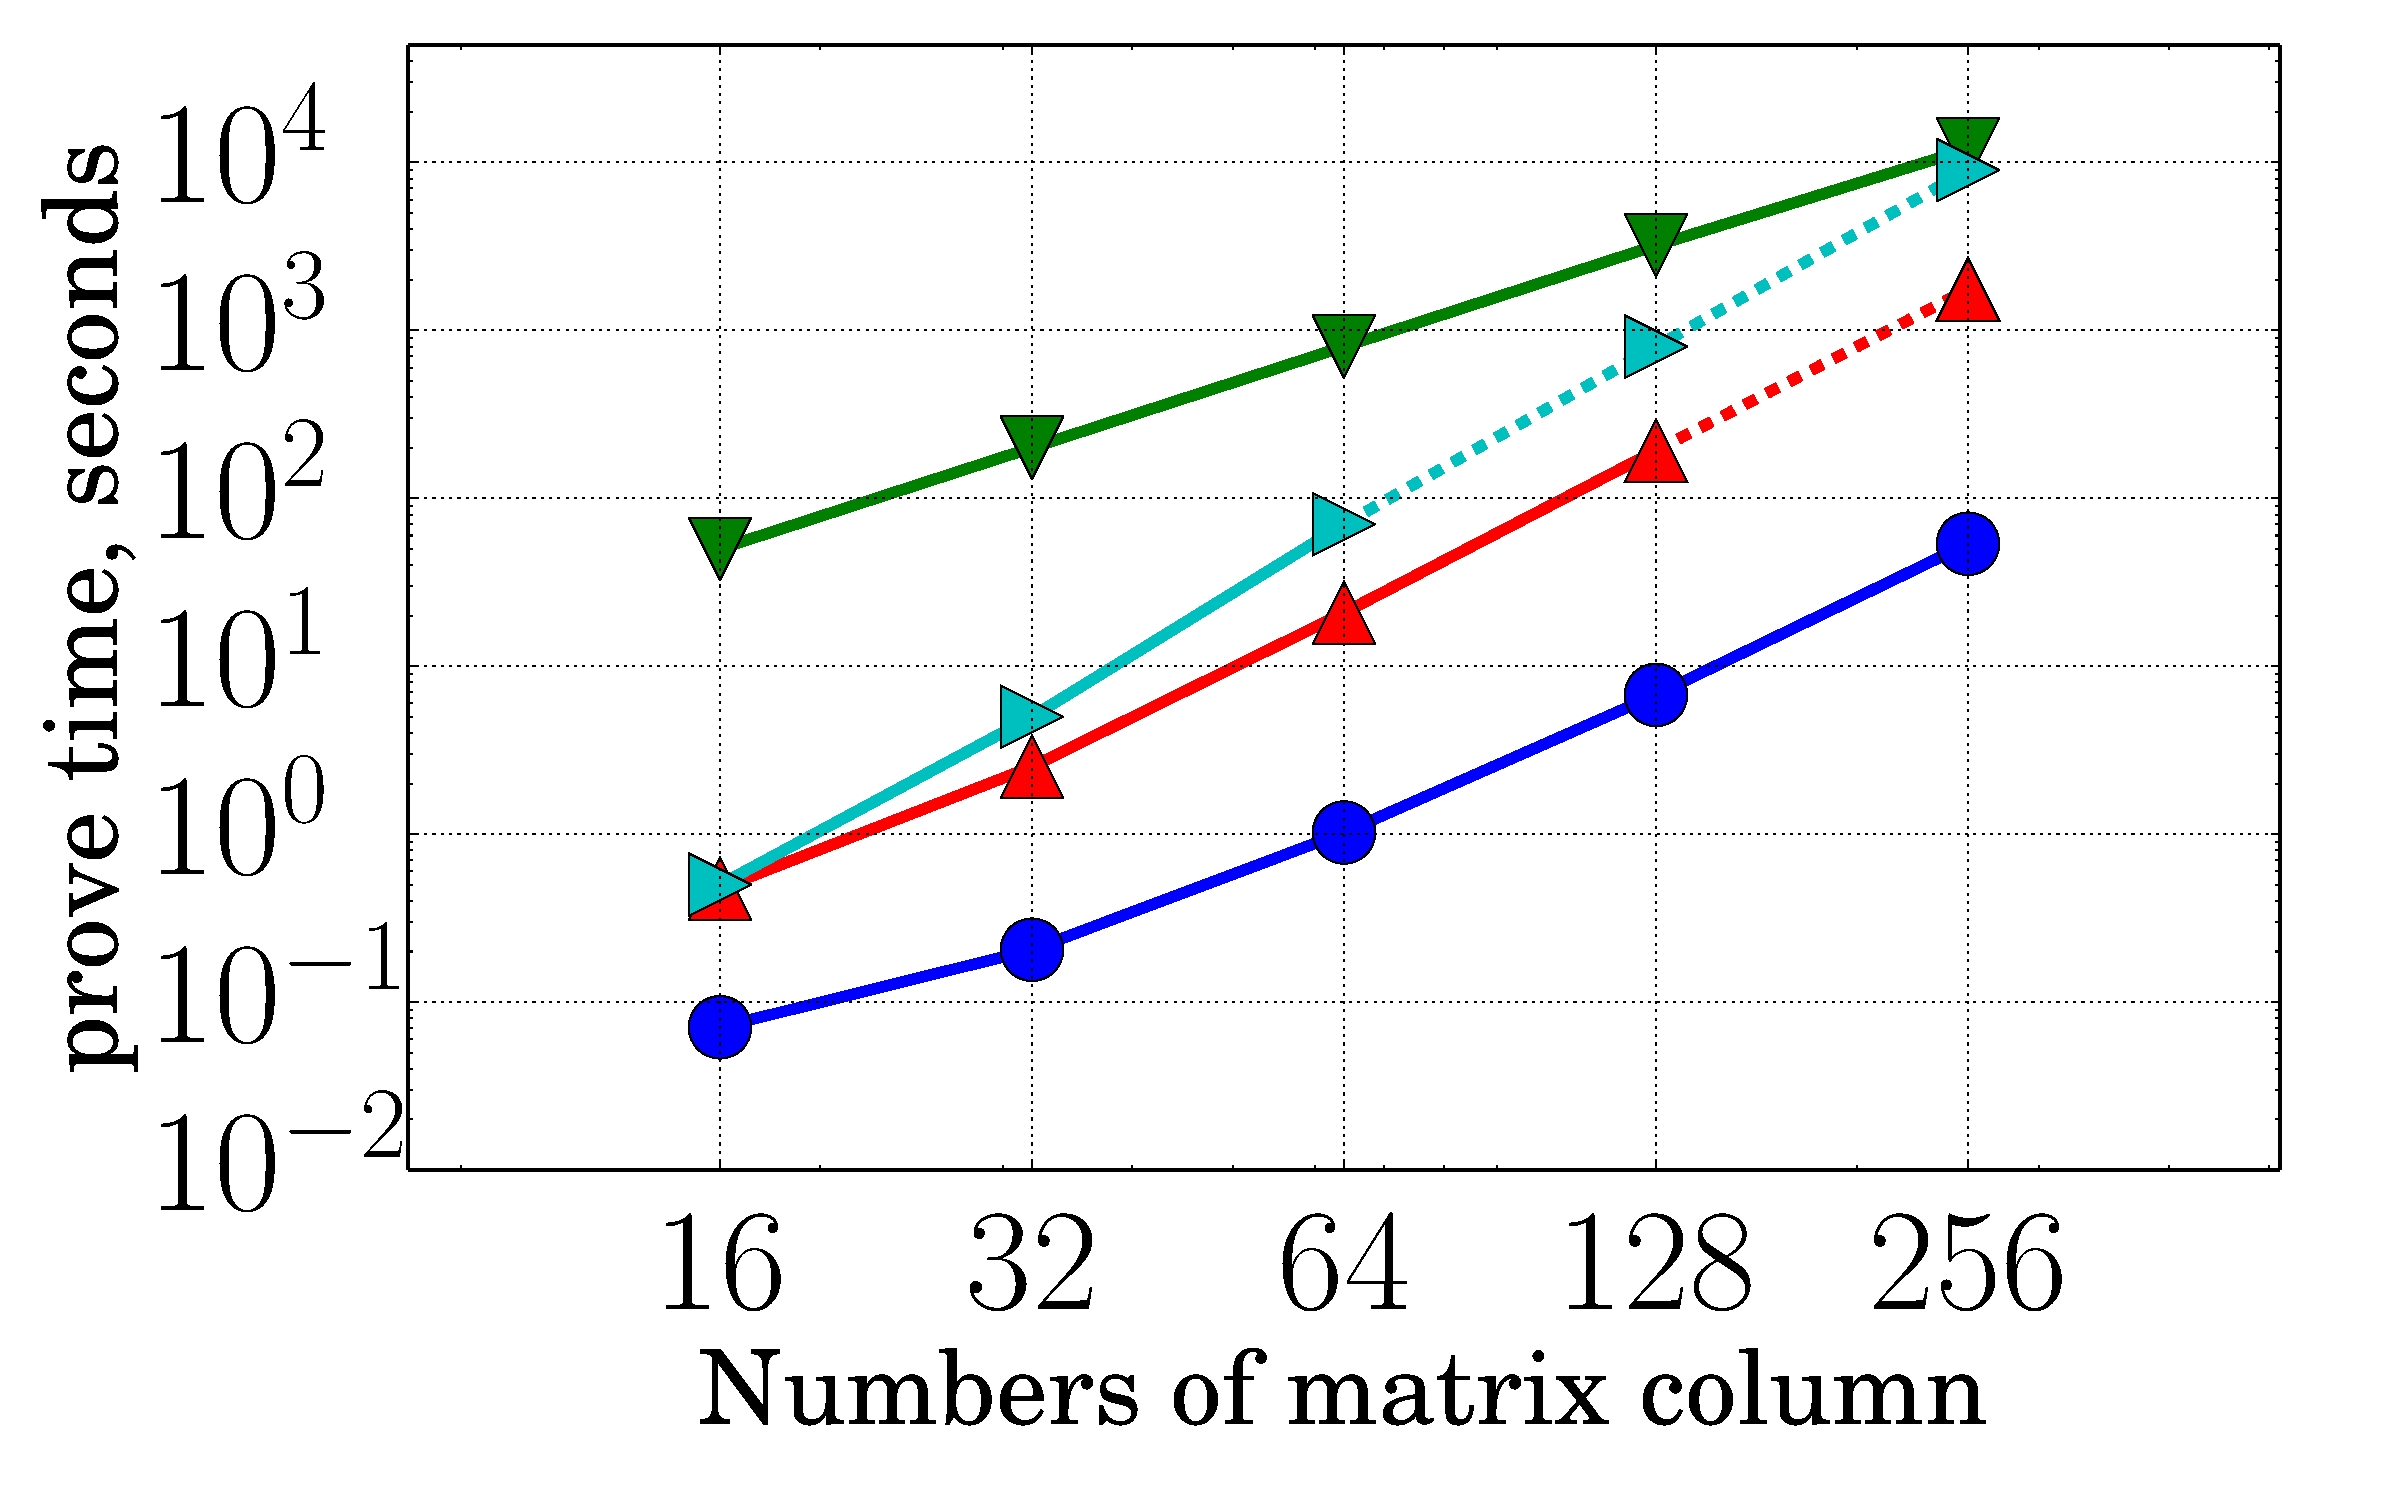
\includegraphics[width=1.5in]{fig4.pdf}
%\caption{fig2}
%\end{minipage}
}%
%\hspace{0.65in}
\subfigure[$\mathcal{P}$ time: 16x Lanczos]{
%\begin{minipage}[t]{0.25\linewidth}
%\centering
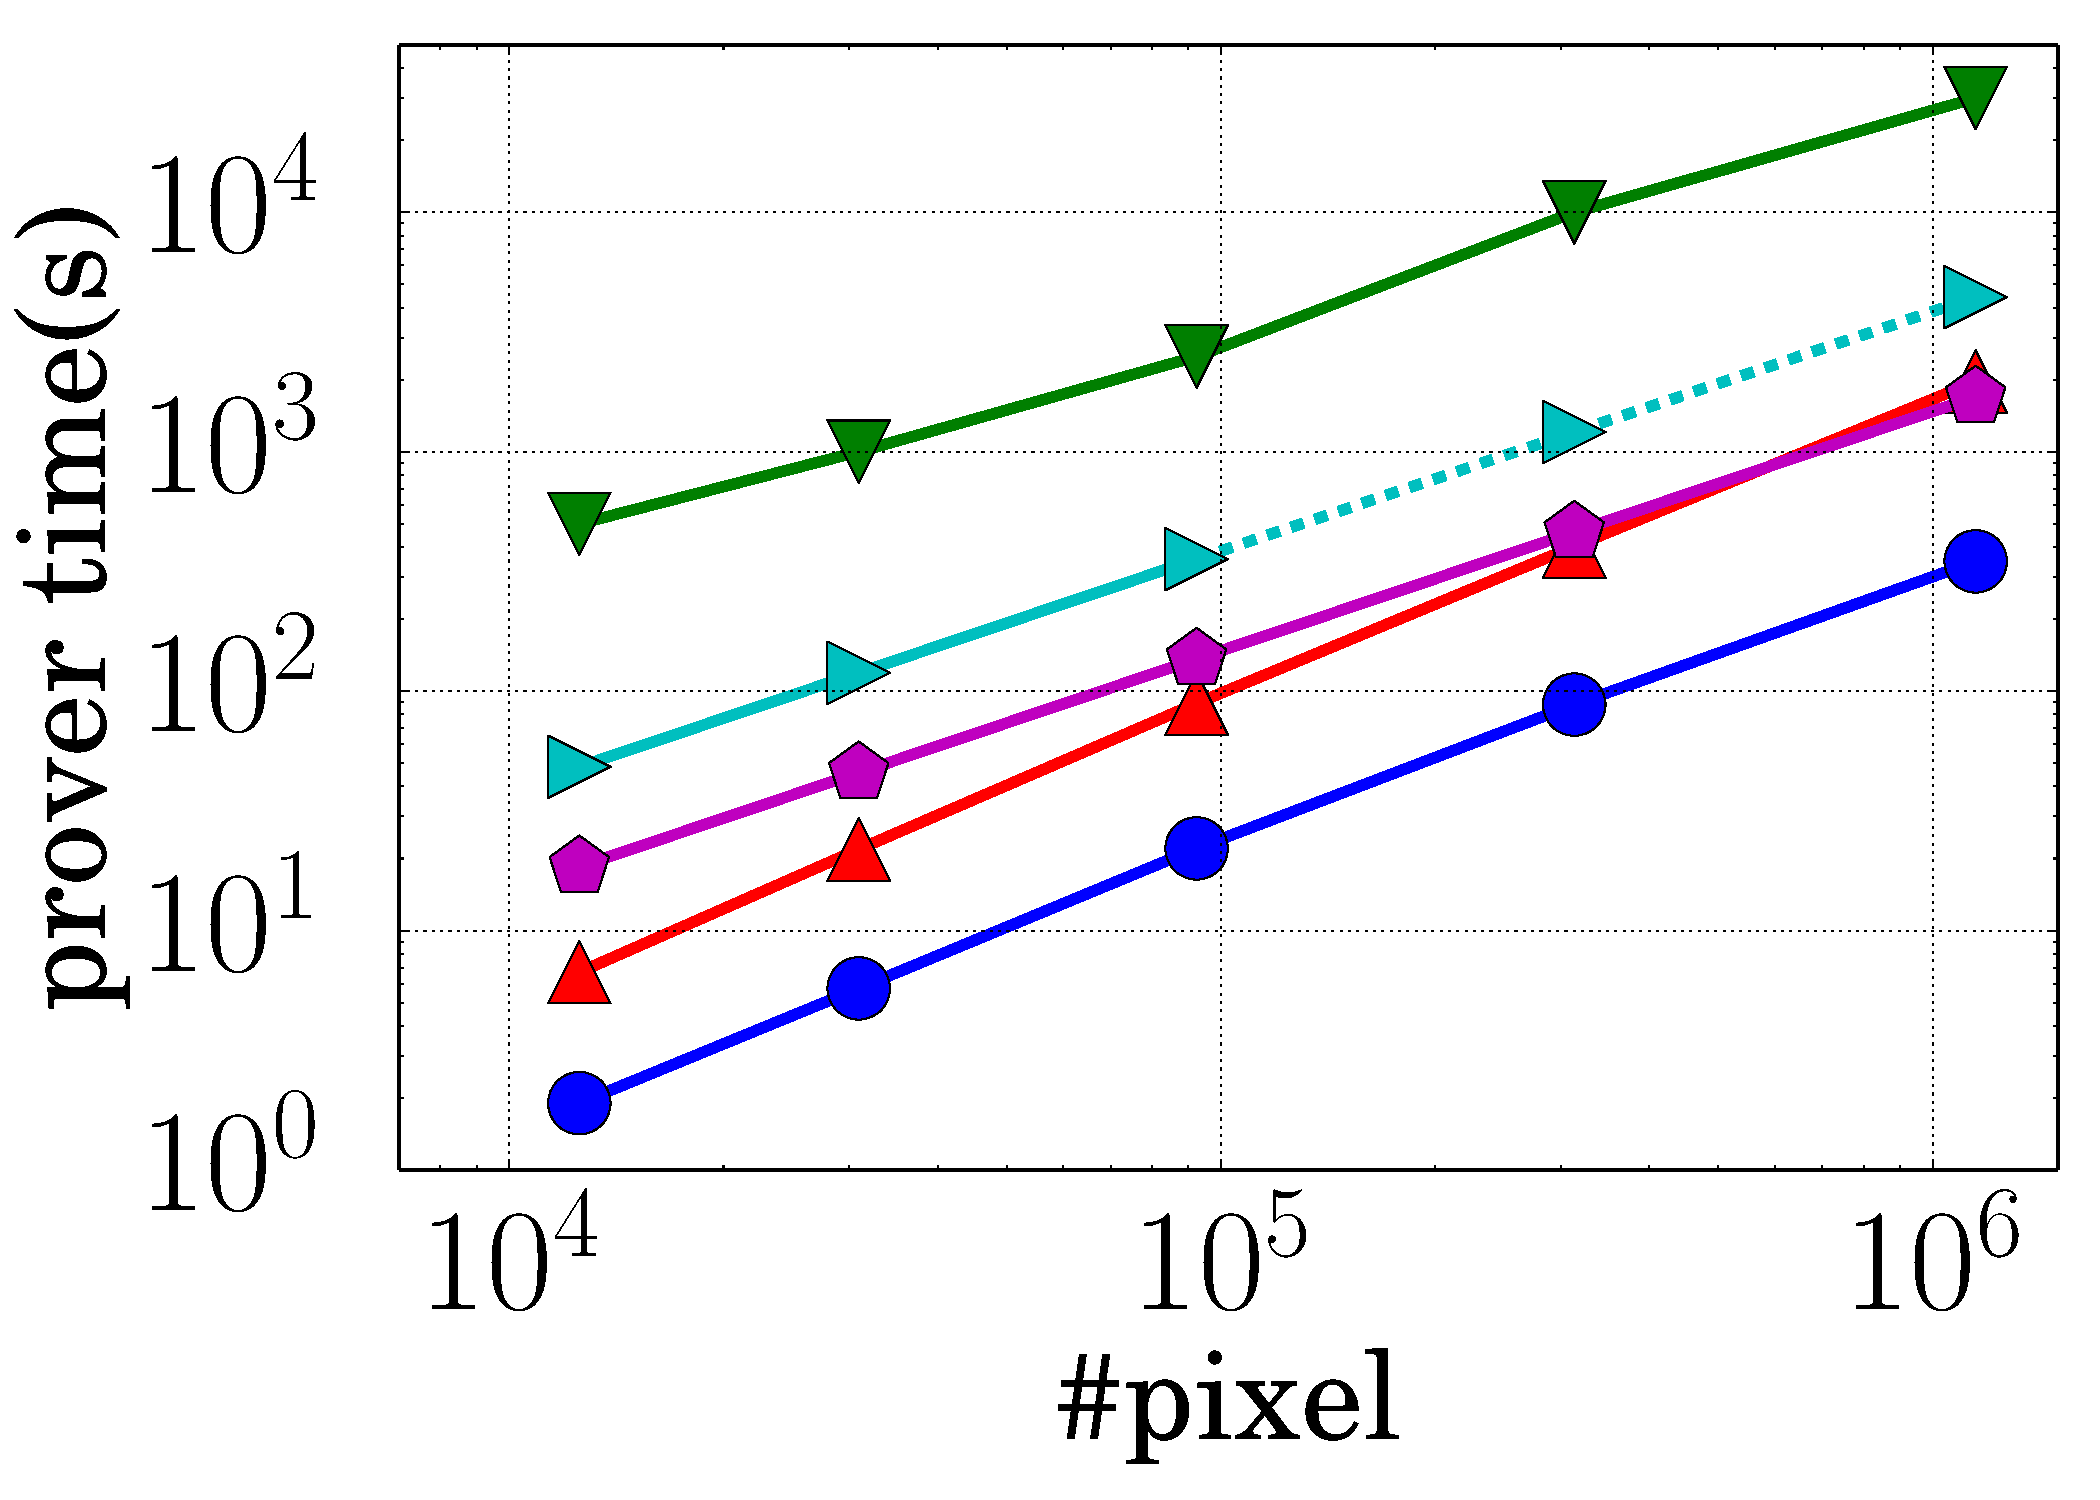
\includegraphics[width=1.5in]{fig5.pdf}
%\caption{fig2}`
%\end{minipage}
}%
%\hspace{0.65in}
\subfigure[$\mathcal{P}$ time: Merkle tree]{
%\begin{minipage}[t]{0.25\linewidth}
%\centering
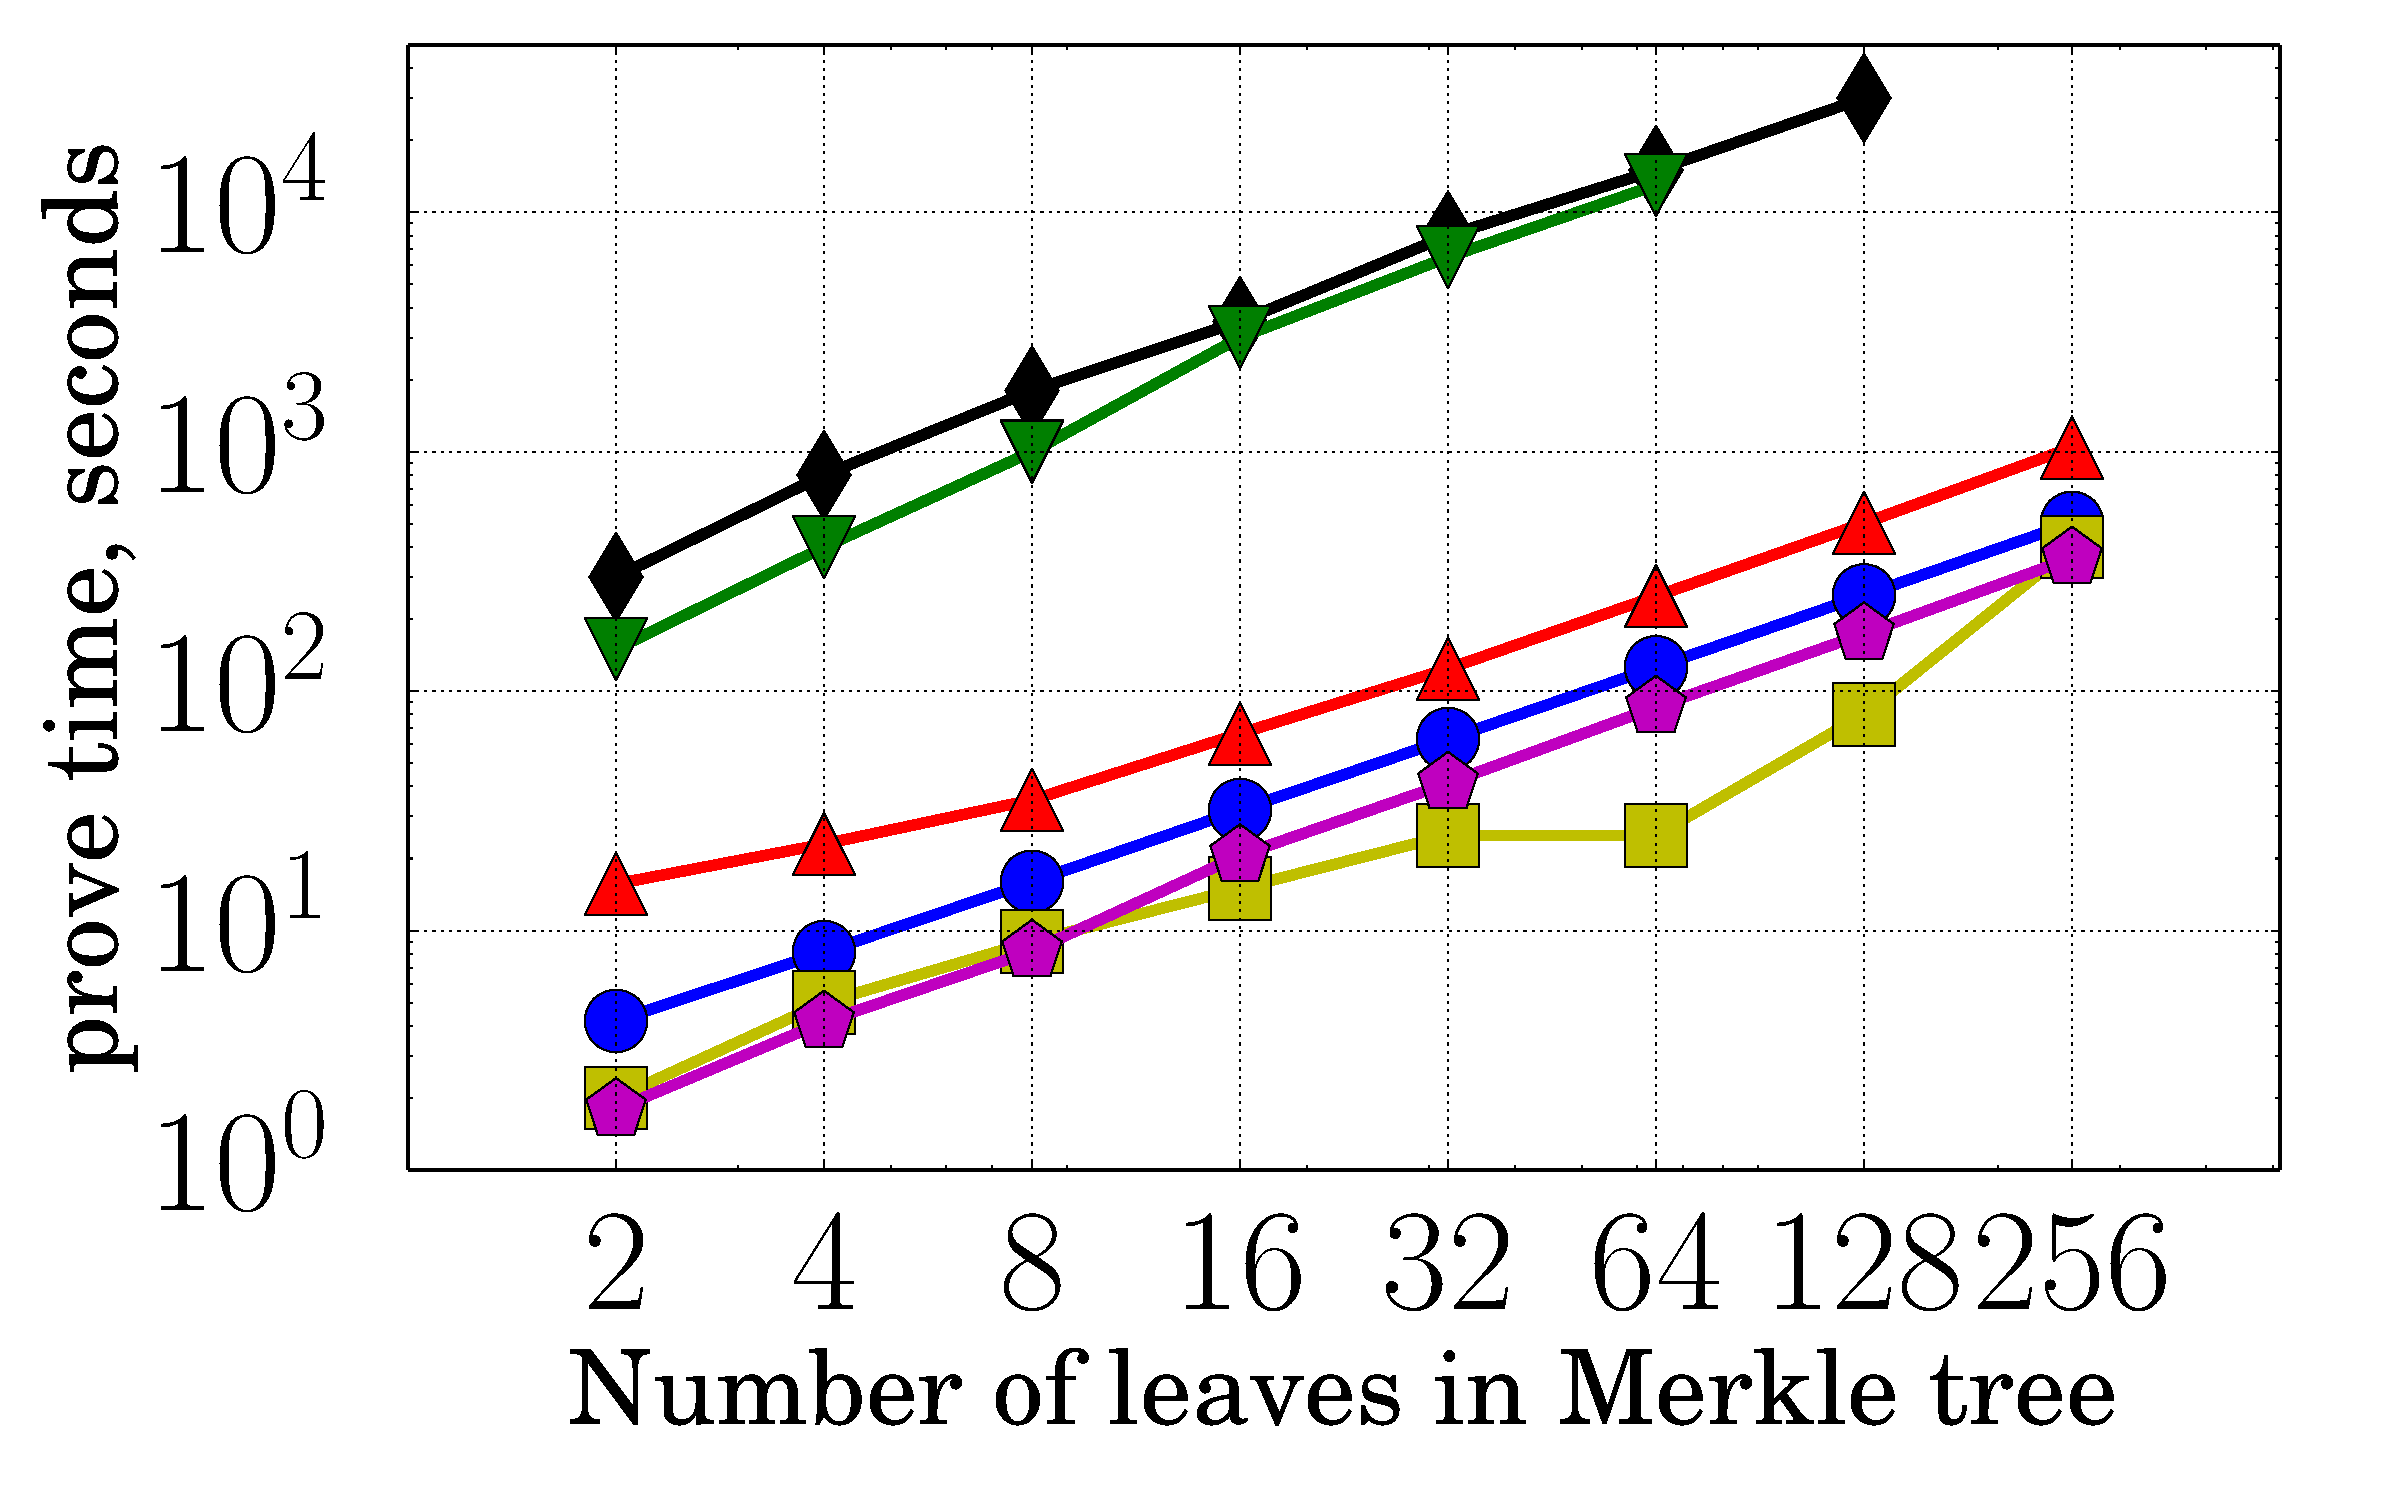
\includegraphics[width=1.5in]{fig6.pdf}
%\caption{fig2}`
%\end{minipage}
}%
\quad  
\subfigure[$\mathcal{V}$ time: MatMul.]{
	%\begin{minipage}[t]{0.25\linewidth}
	%\centering
	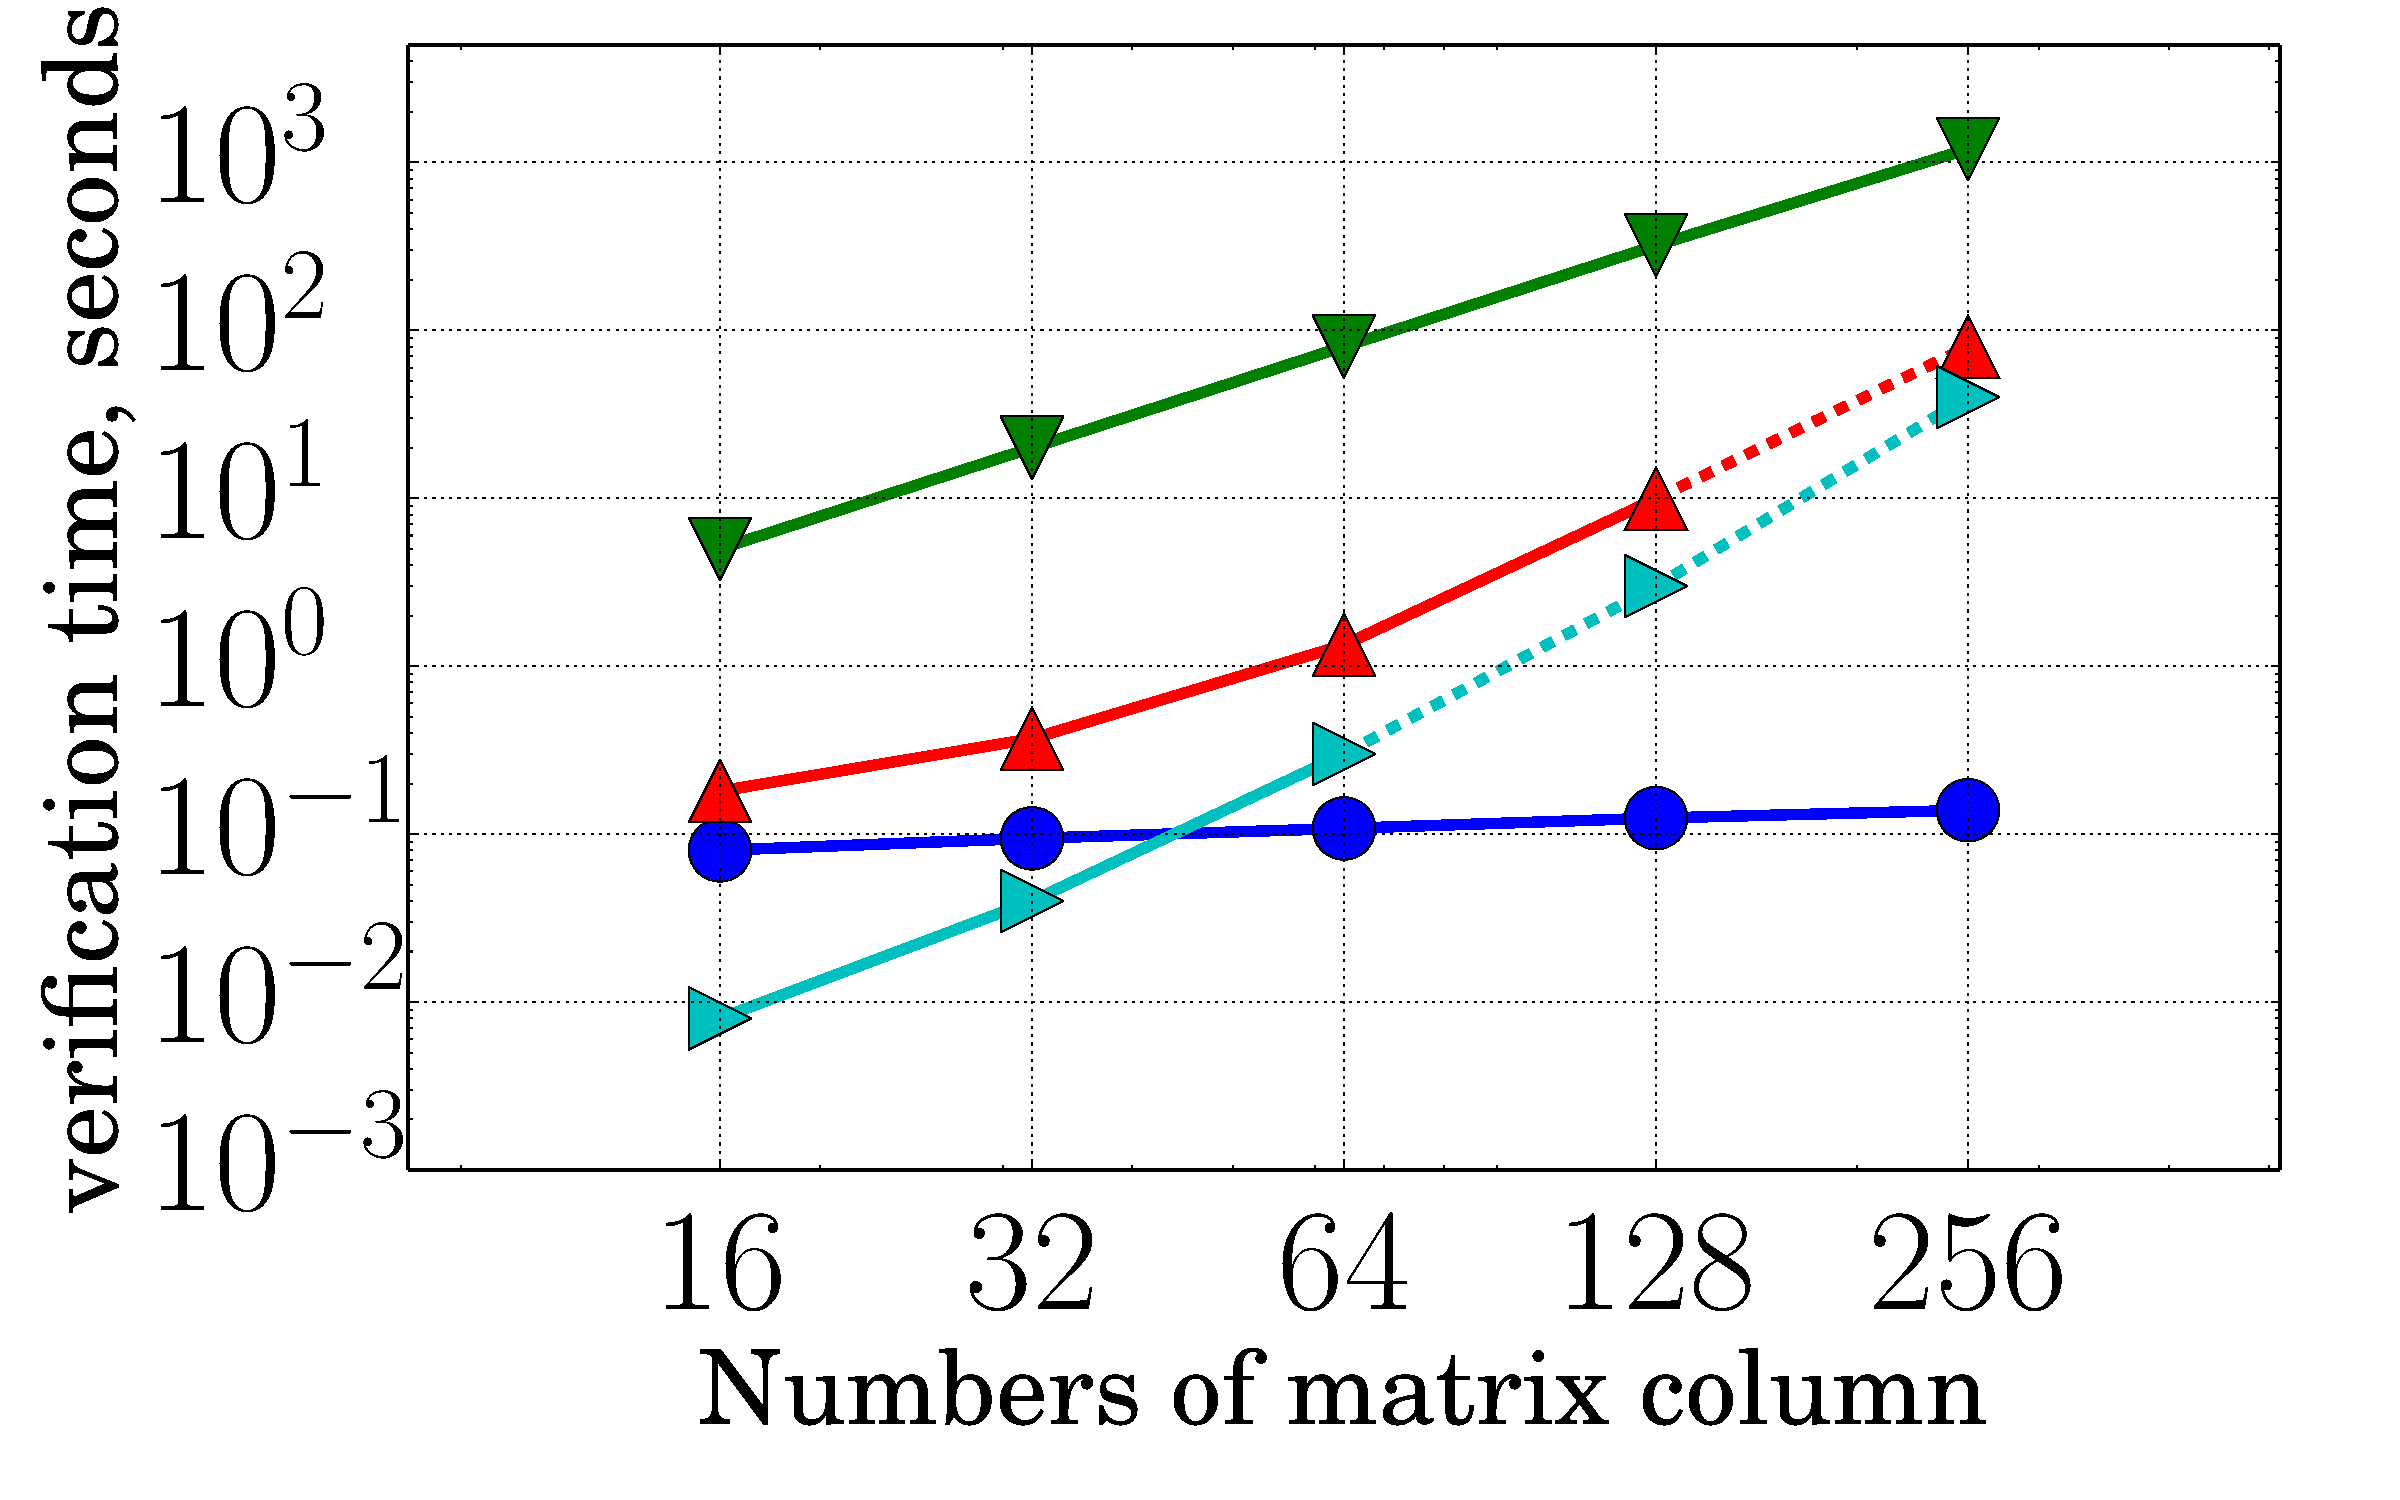
\includegraphics[width=1.5in]{fig7.pdf}
	%\caption{fig2}
	%\end{minipage}
}%
%\hspace{0.65in}
\subfigure[$\mathcal{V}$ time: 16x Lanczos]{
	%\begin{minipage}[t]{0.25\linewidth}
	%\centering
	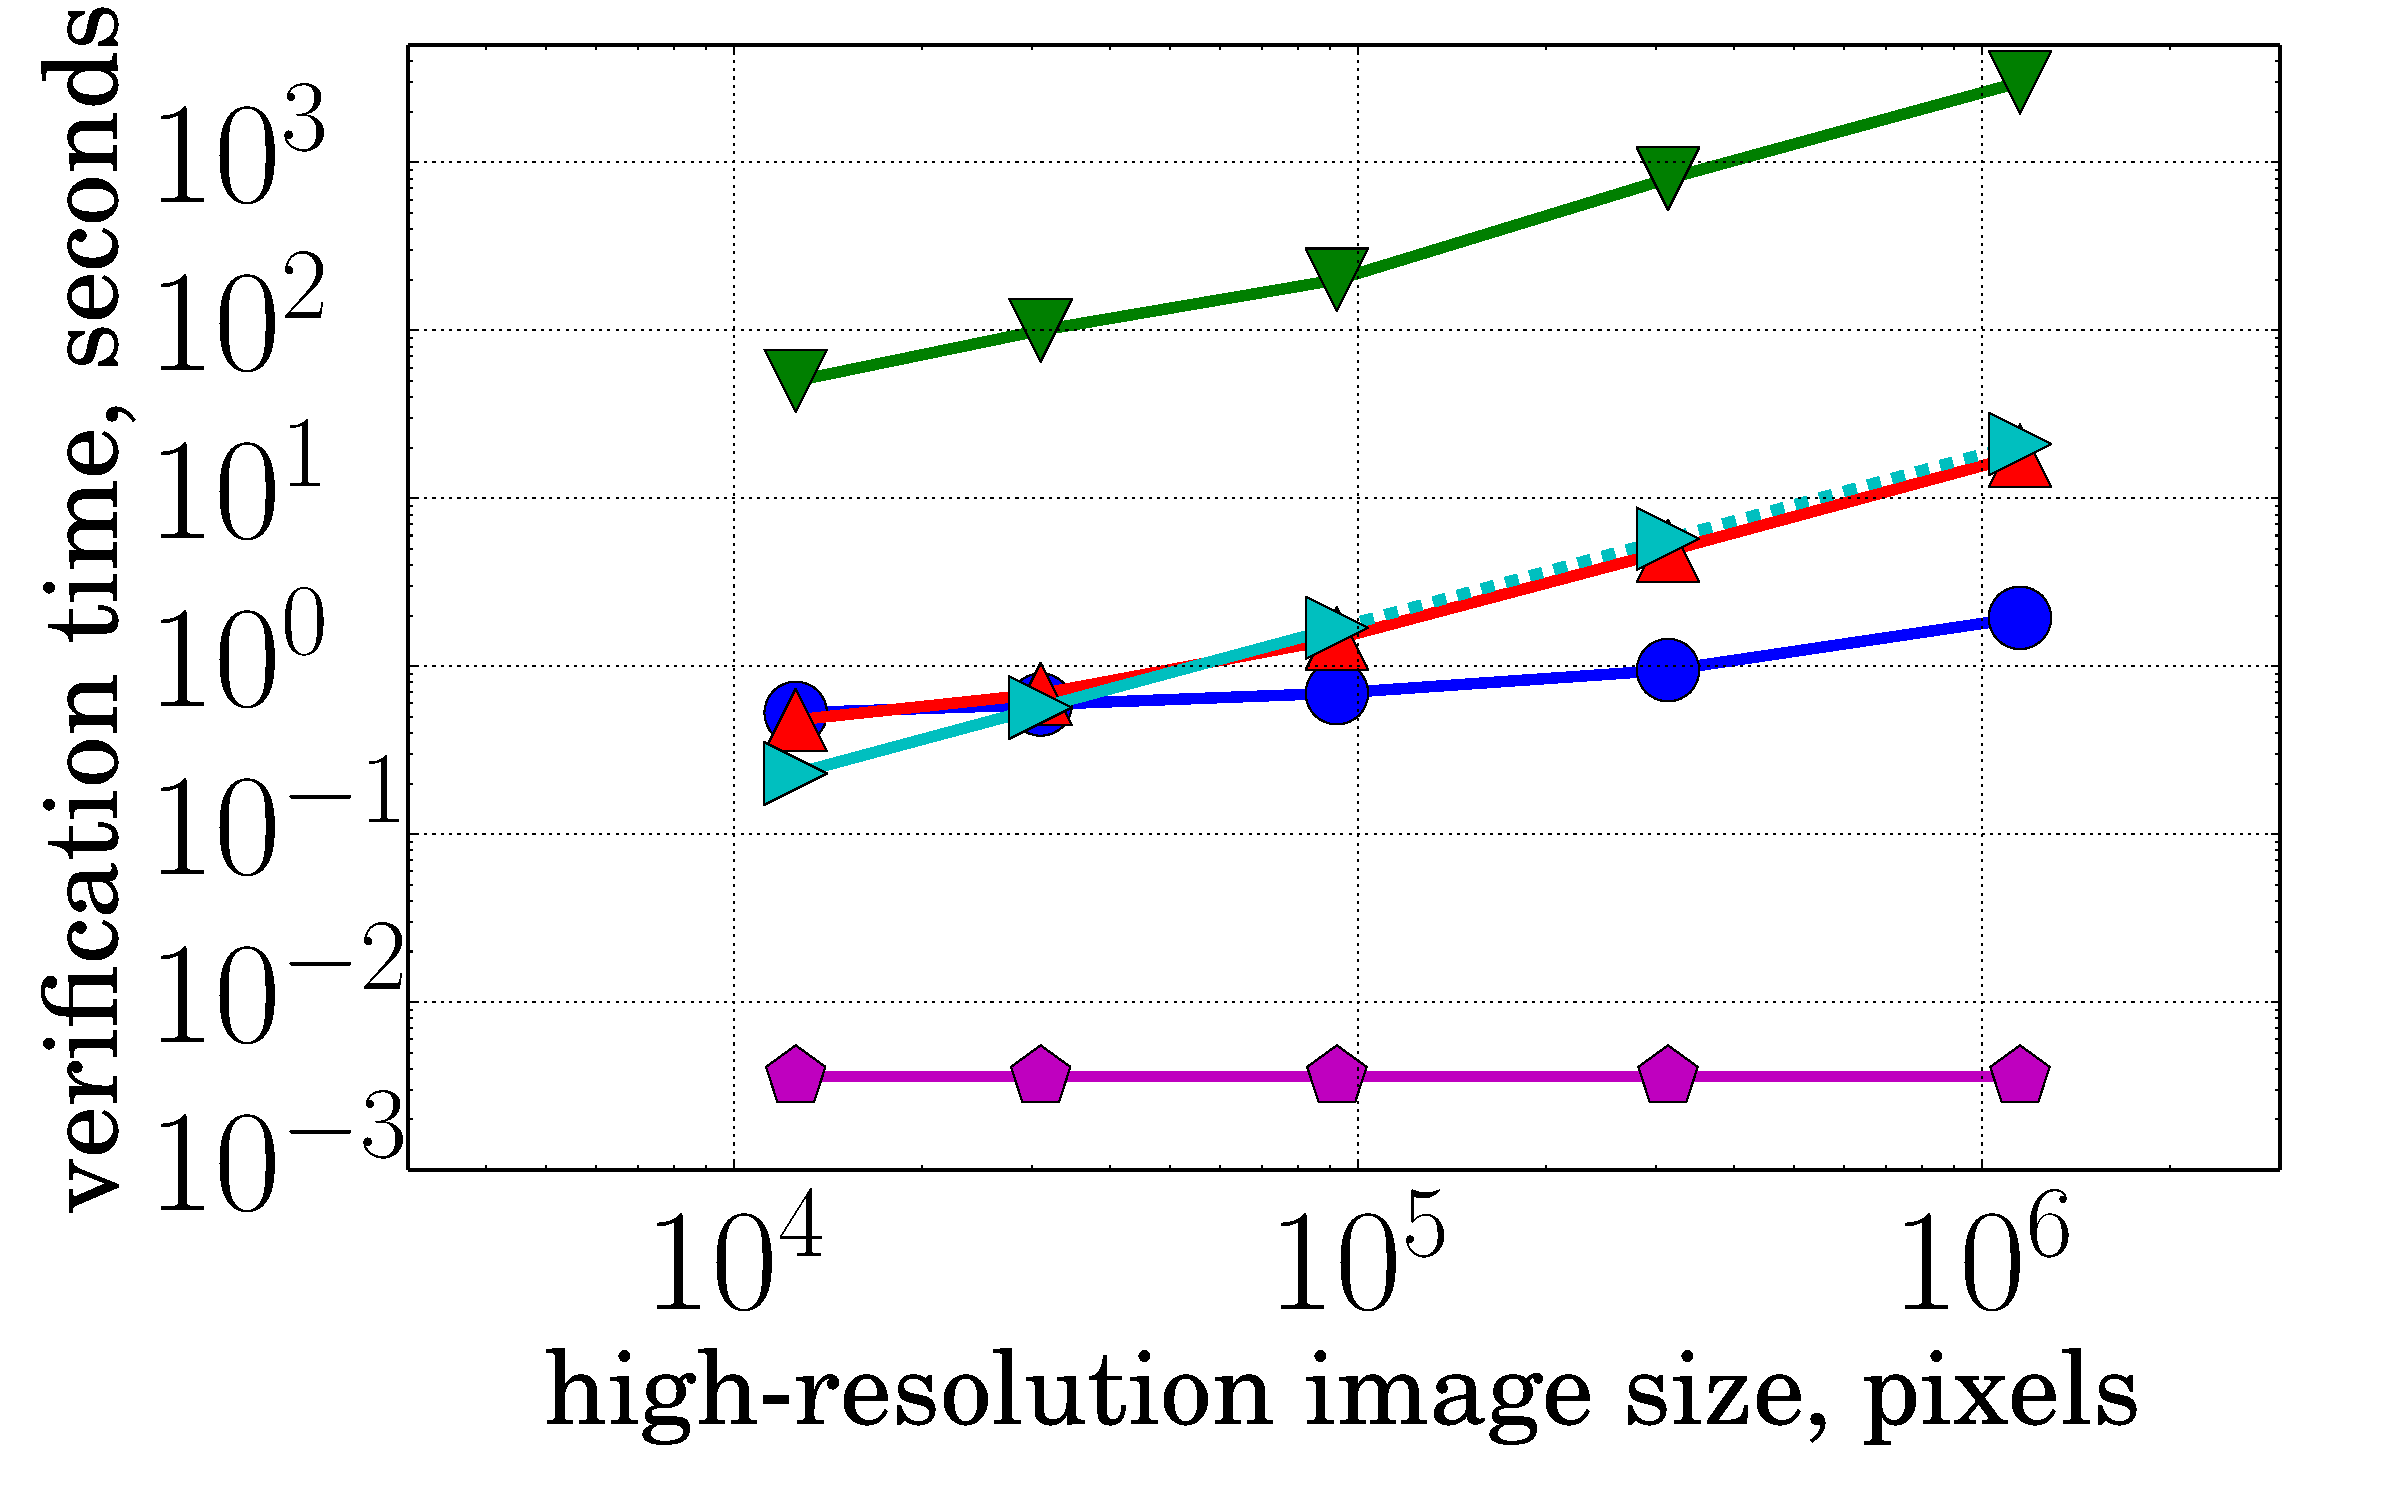
\includegraphics[width=1.5in]{fig8.pdf}
	%\caption{fig2}`
	%\end{minipage}
}%
%\hspace{0.65in}
\subfigure[$\mathcal{V}$ time: Merkle tree]{
	%\begin{minipage}[t]{0.25\linewidth}
	%\centering
	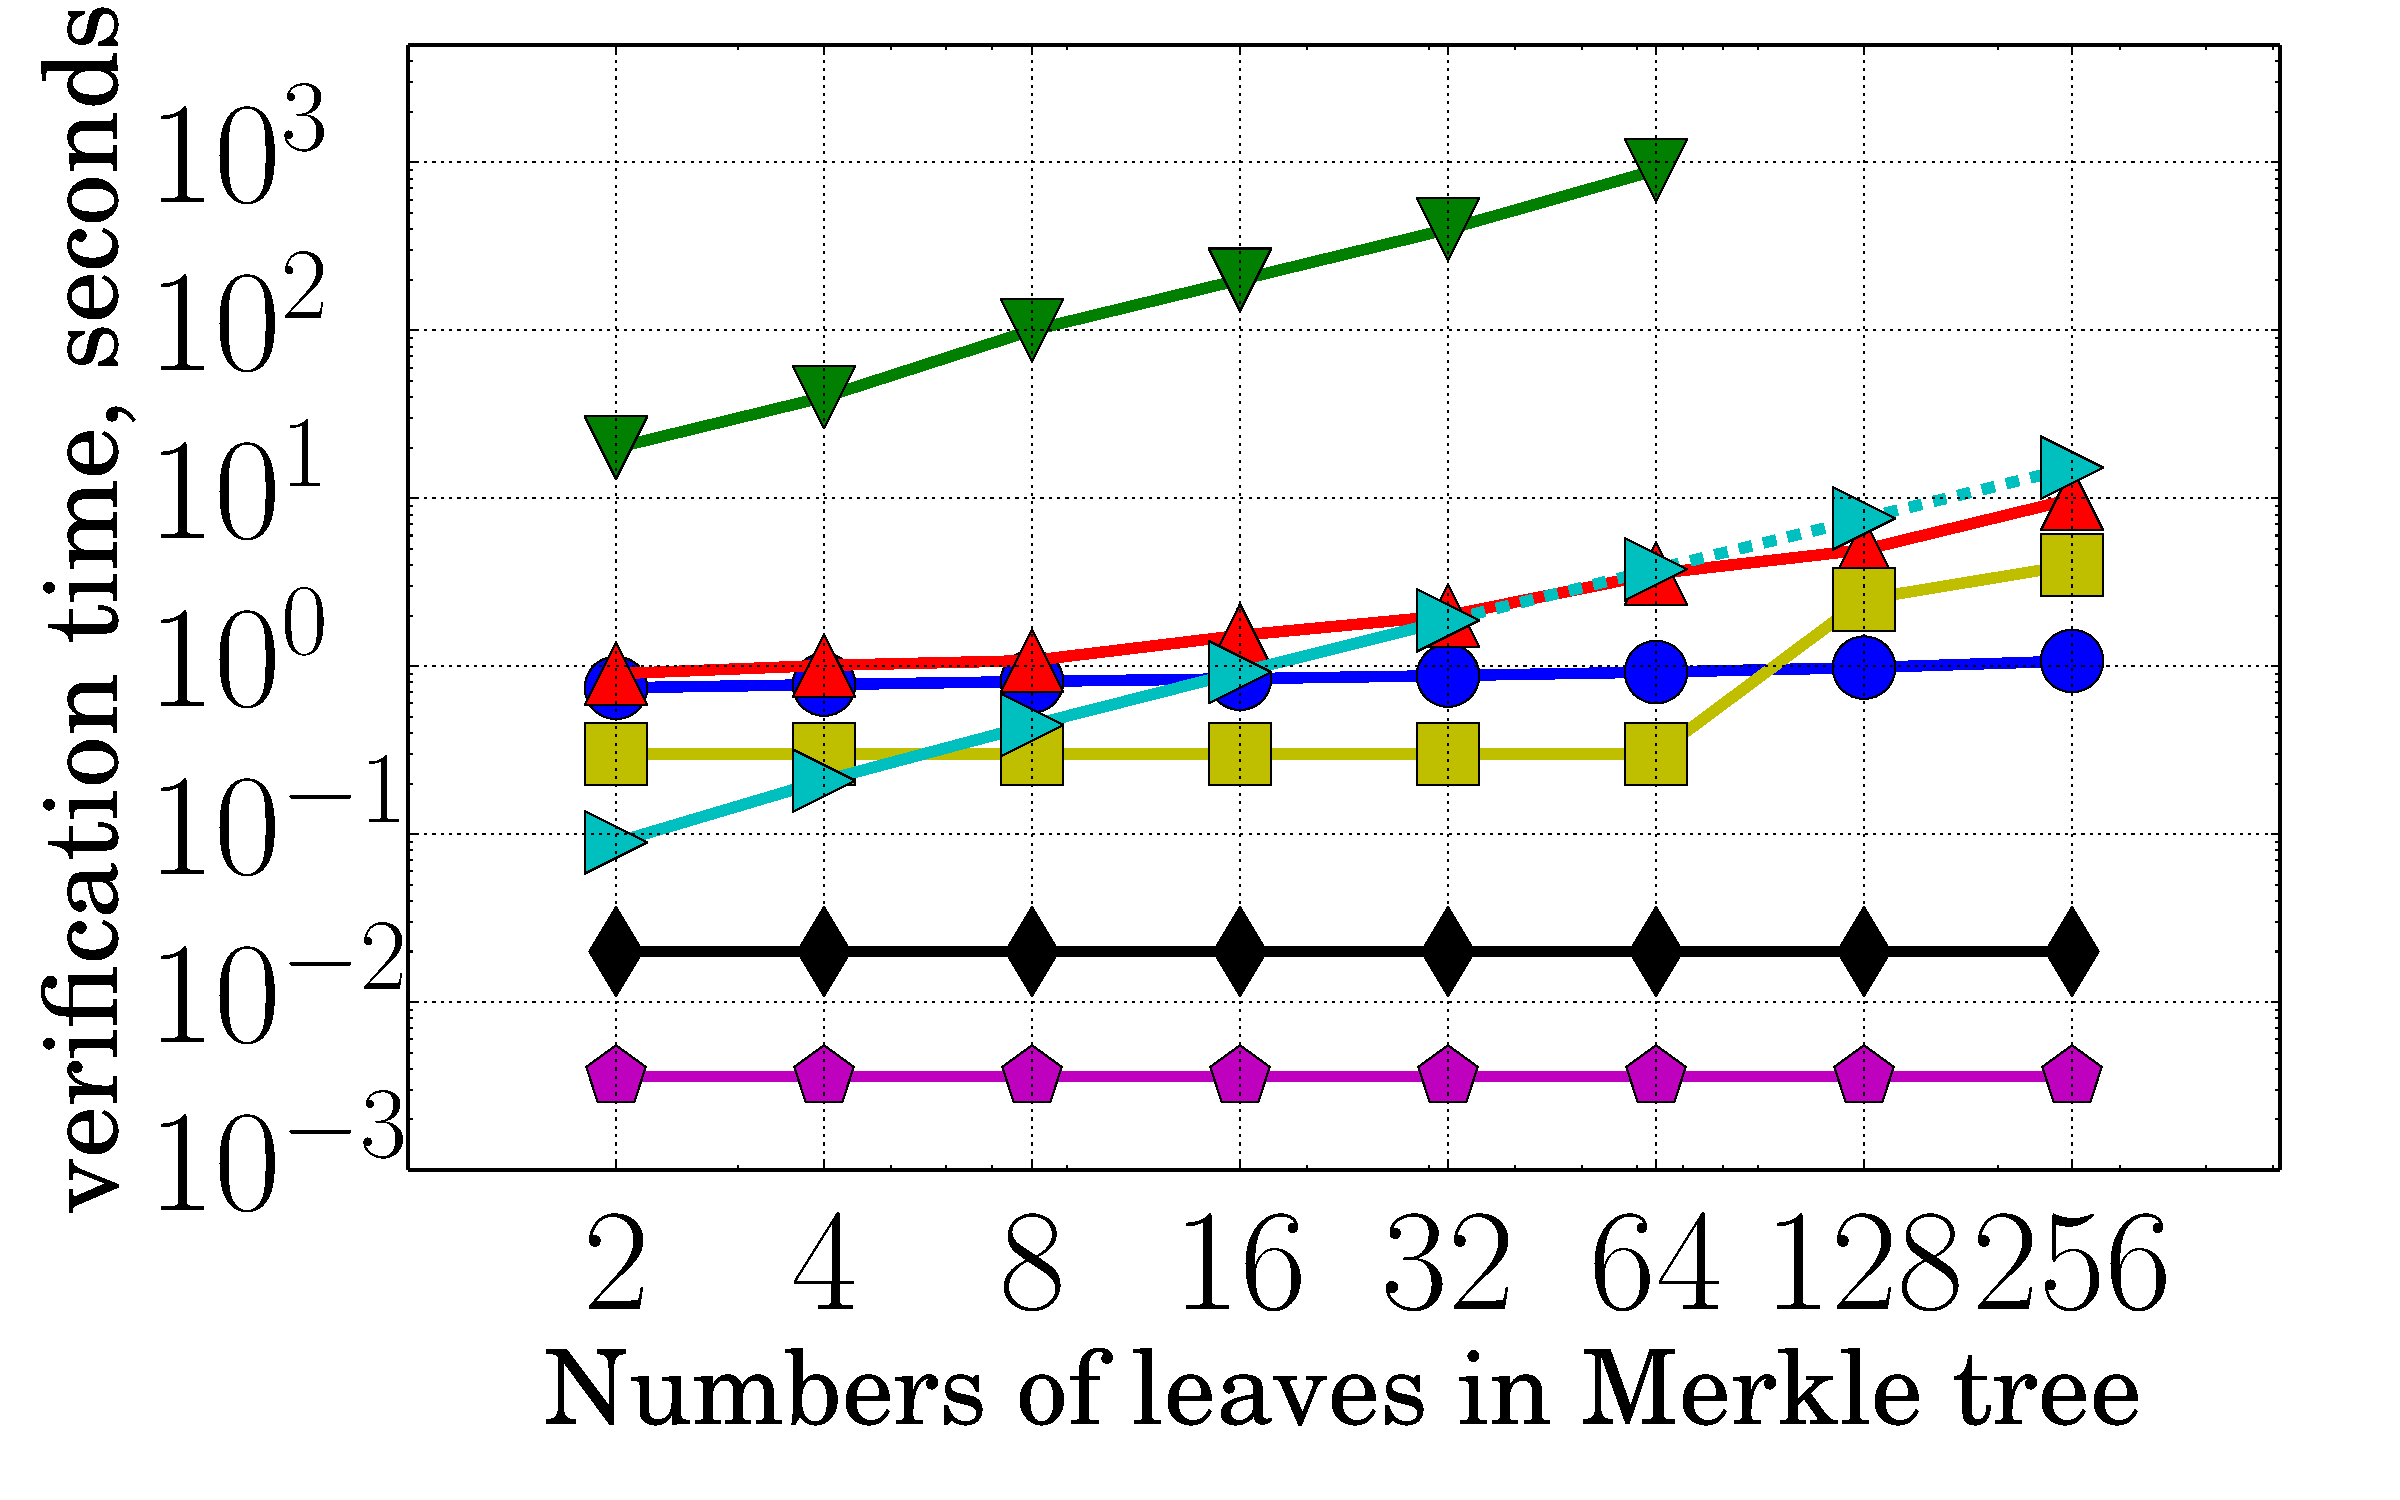
\includegraphics[width=1.5in]{fig9.pdf}
	%\caption{fig2}`
	%\end{minipage}
}% 
\quad        
%\centering
\subfigure[Proof size: MatMul.]{
	%\begin{minipage}[t]{0.25\linewidth}
	\centering
	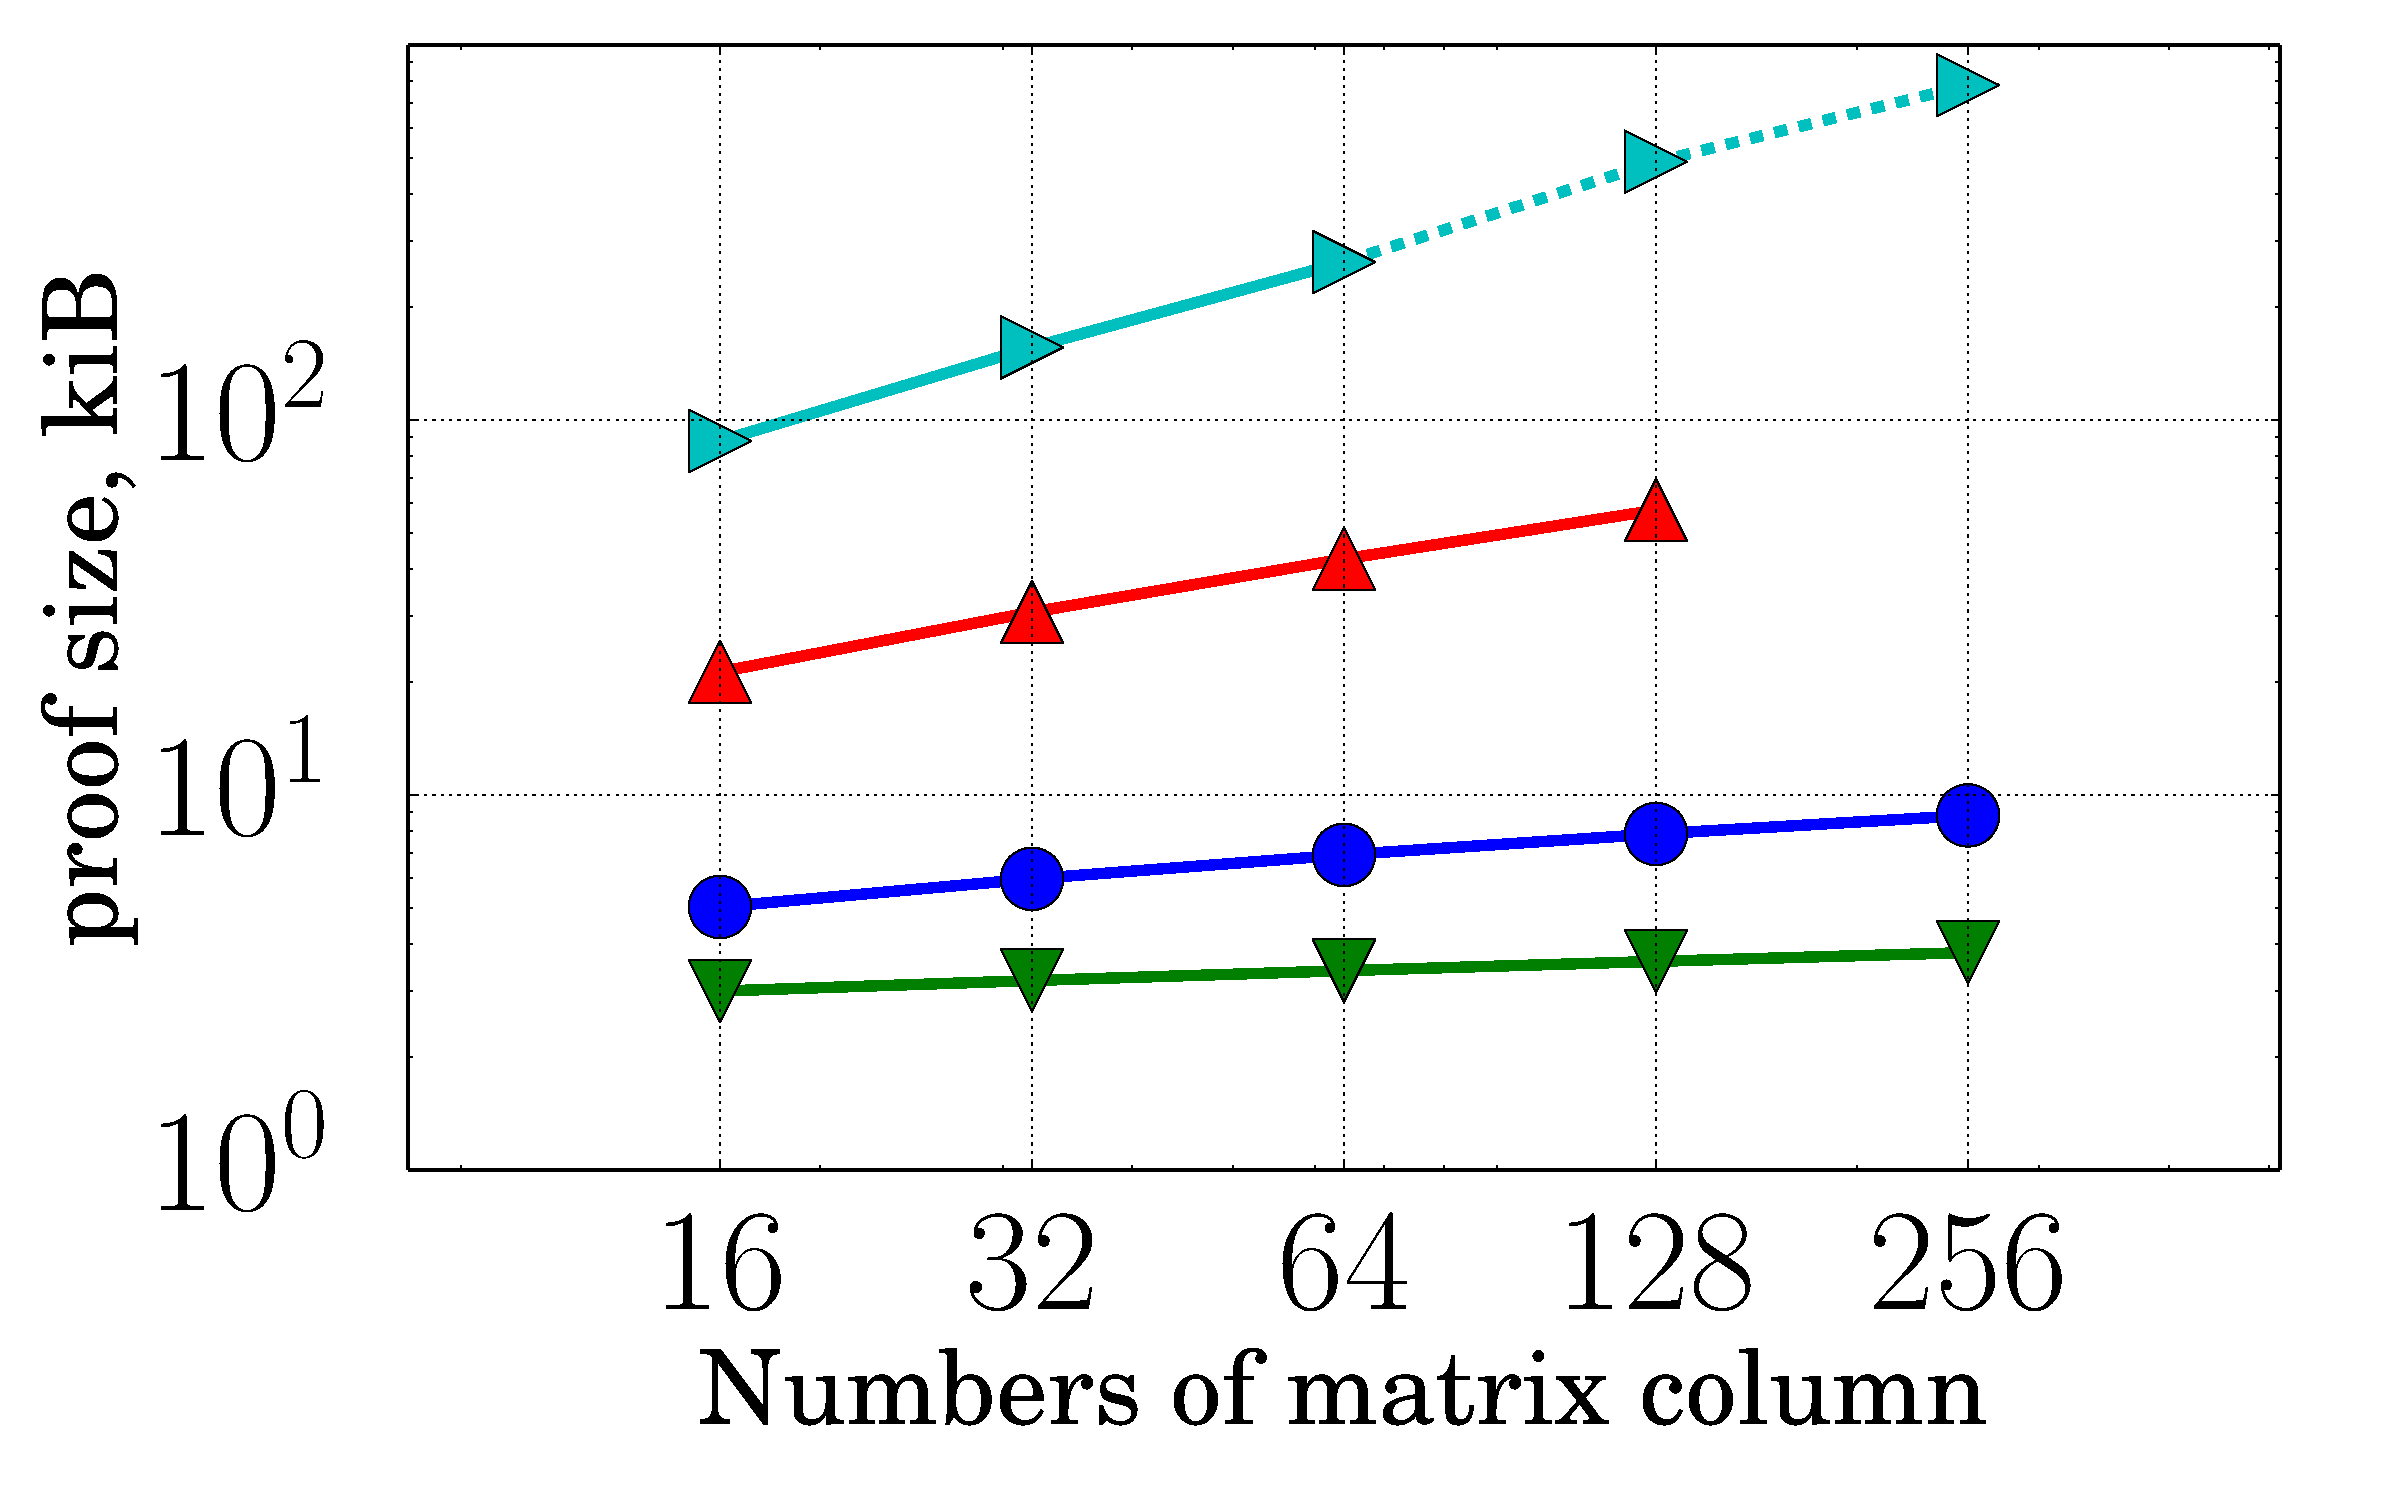
\includegraphics[width=1.5in]{fig1.pdf}
	%\caption{fig1}
	%\end{minipage}%
}%
%\hspace{0.05in}
\subfigure[Proof size: 16x Lanczos]{
	%\begin{minipage}[t]{0.25\linewidth}
	%\centering
	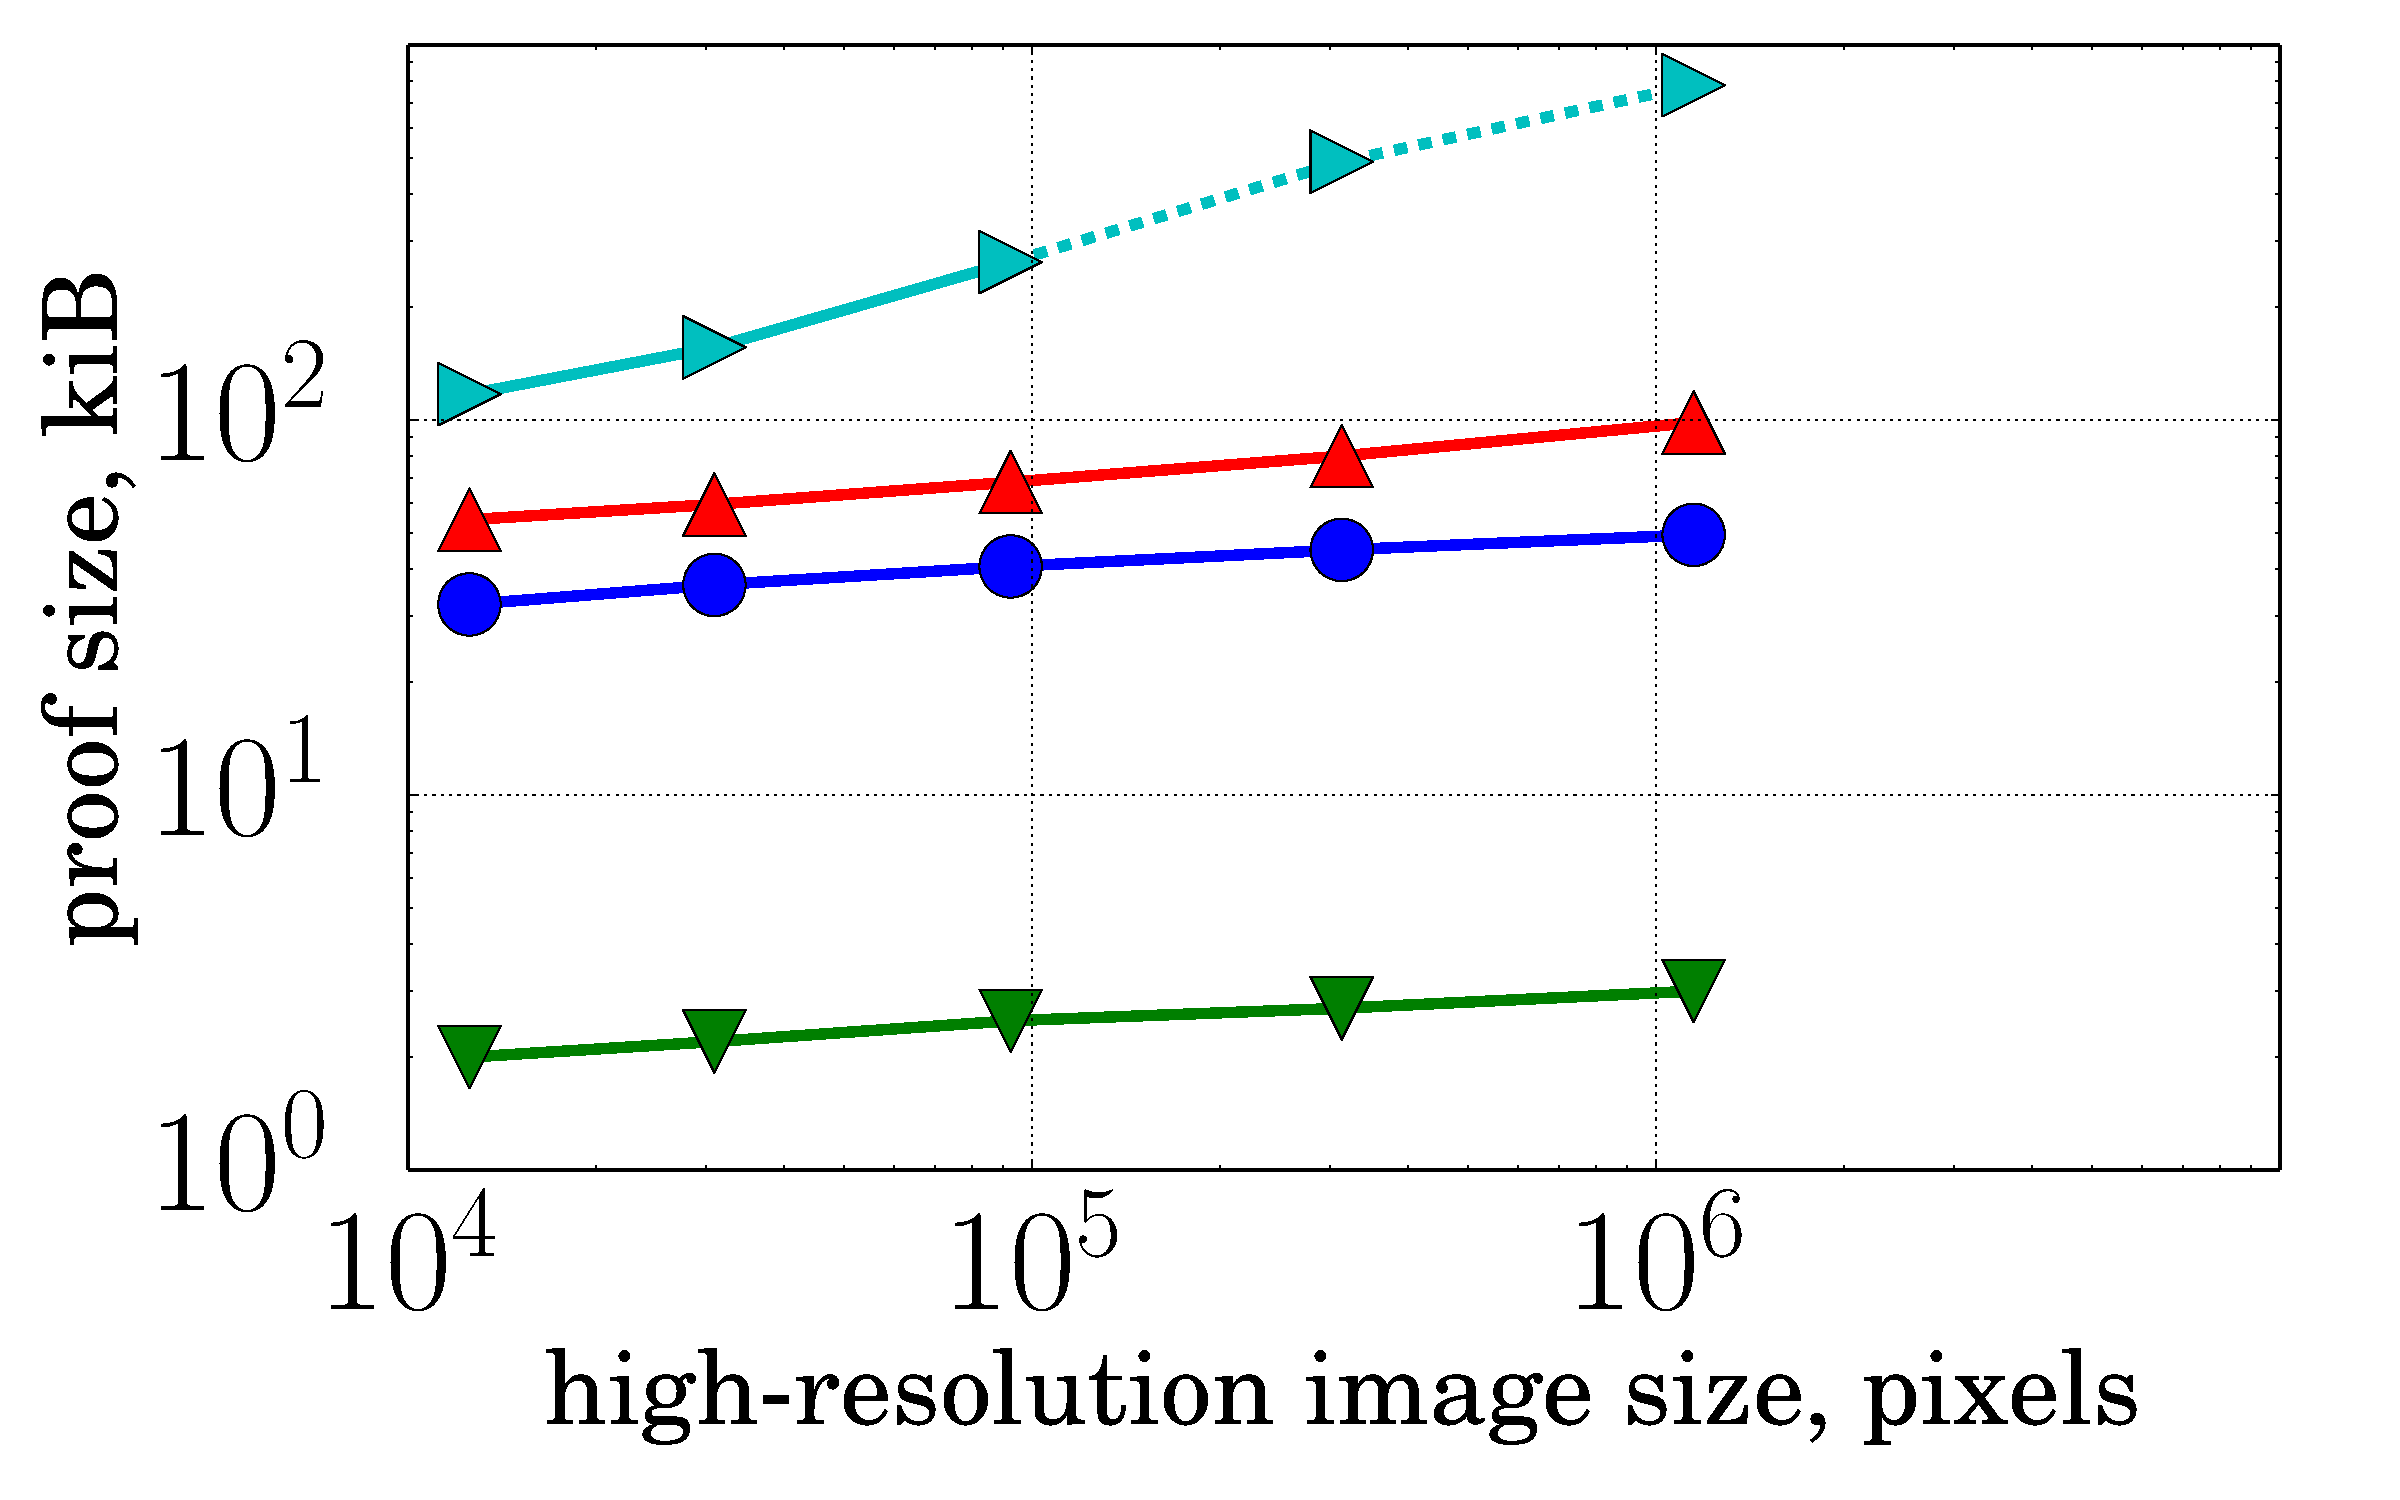
\includegraphics[width=1.5in]{fig2.pdf}
	%\caption{fig2}
	%\end{minipage}%
}%
%\hspace{0.05in}
\subfigure[Proof size: Merkle tree]{
	%\begin{minipage}[t]{0.25\linewidth}
	%\centering
	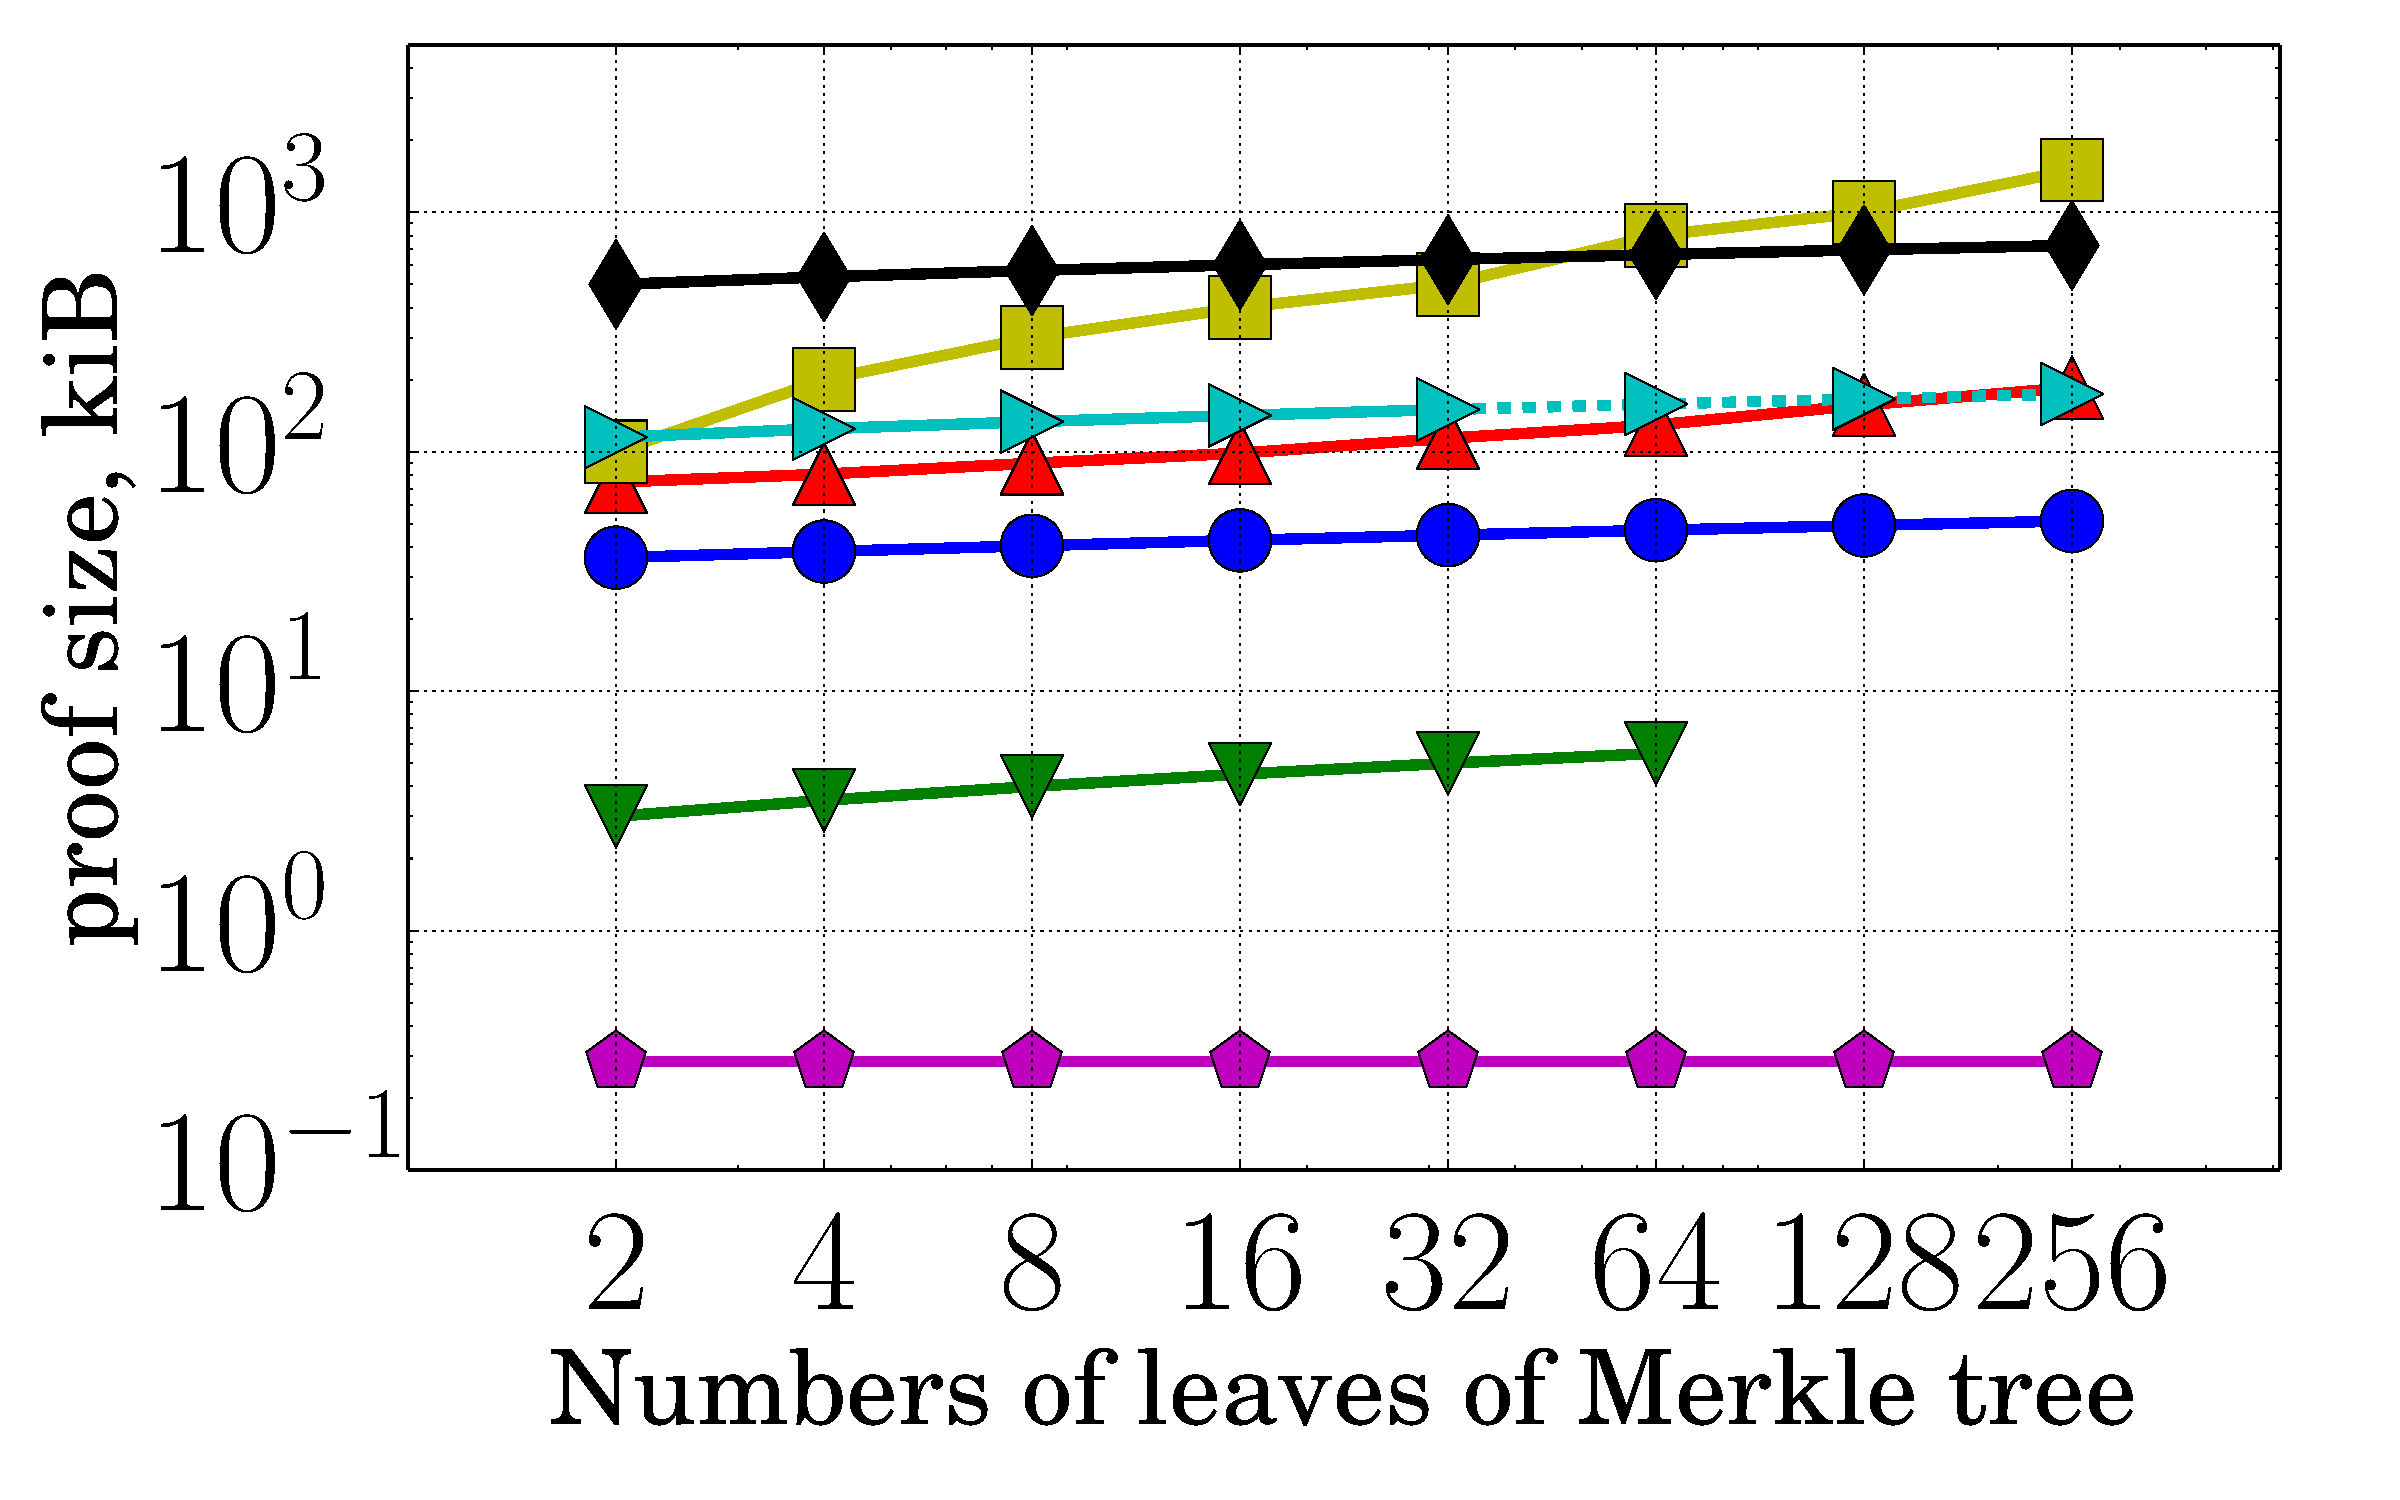
\includegraphics[width=1.5in]{fig3.pdf}
	%\caption{fig2}
	%\end{minipage}%
}%
\quad
\centering

\includegraphics[width = 5in]{legend.pdf}
\caption{\label{fig:Allcom}Comparisons of prover time, proof size and verification time between \name{} and existing zero knowledge proof systems.}
\end{figure}


\paragraph{Prover time.} As shown in Figure~\ref{fig:Allcom}(a)(b)(c), the prover in \name is the fastest among all systems in all three benchmarks we tested. Ligero is one of the best existing ZKP systems on prover time as it is purely based on symmetric key operations. Comparing to Ligero, the prover time of \name is $1.15\times$ faster on a Merkle tree with 2 leaves and $2\times$ faster with 256 leaves. Comparing to other systems, \name improves the prover time by $3.4-8.9\times$ vs. Hyrax, by $7.1-16.1\times$ vs. Aurora, by $65-166\times$ vs. Bulletproof and by $150-170\times$ vs. libSTARK. 

\name is also faster than libSNARK on general circuits by $5-10\times$, as shown in Figure~\ref{fig:Allcom}(a) and~\ref{fig:Allcom}(b). The performance of \name is comparable to libSNARK on Merkle trees in Figure~\ref{fig:Allcom}(c). This is because (1) most values in the circuit of SHA256 are binary, which is friendly to the prover of libSNARK as the time of exponentiations is proportional to the bit-length of the values; (2) The R1CS of SHA256 is highly optimized by jsnark~\cite{jsnark} and real world products like Zcash~\cite{zerocash}. There are only 26,000 constrains in one hash. In the arithmetic circuit used by \name, there are 60,000 gates with 38,000 of them being multiplication gates. Even so, \name is still as fast as libSNARK on a Merkle tree with 2 leaves and $2\times$ faster with 256 leaves. We plan to further optimize the implementation of SHA256 as an arithmetic circuit in the future.

The gap between \name and other systems will become bigger as the size of the circuit grows, as the prover time in these systems (other than Bulletproof) scales quasi-linearly with the circuit size. The experimental results justify that the prover time in \name is both optimal asymptotically, and efficient in practice.

\paragraph{Verification time.} Figure~\ref{fig:Allcom}(d)(e)(f) show the verification time. Our verifier is much slower than libSNARK and libSTARK, which runs in 3ms and 10-30ms respectively in all the benchmarks. 

Other than these two systems, the verification time of \name is faster, as it grows sub-linearly with the circuit size. In particular, our verification time ranges from $0.08-1.15$s in the benchmarks we consider. In Figure~\ref{fig:Allcom}(f), the verification time of \name is $8\times$ slower than Aurora when $M=2$, and $15\times$ faster when $M=256$. \name is $2.5\times$ slower than Ligero with $M=2$ and $4\times$ faster with $M=256$. Comparing to Hyrax and Bulletproof, our verification is $1.2-9\times$ and $27-900\times$ faster respectively. Again, the gap increases with the scale of the circuits as our verification is succinct.

\paragraph{Proof size.} We report the proof size in Figure~\ref{fig:Allcom}(g)(h)(i). Our proof size is much bigger than libSNARK, which is 170 bytes for all circuits, and Bulletproof, which ranges in $2-5.5$KBs. The proof size in \name is in the range of 30-60KBs, except for the matrix multiplications where it reduces to $5-9$KBs. This is better than Aurora, Hyrax and libSTARK, which also have polylogarithmic proof size to the circuit. Finally, the proof size in Ligero is $O(\sqrt{C})$ and grows to several megabytes in practice.

\paragraph{Setup time.} Among all the systems, only \name and libSNARK require trusted setup. Thanks to the optimization described in the beginning of this section, it only takes 202s to generate the public parameters in our largest instance with $n = 2^24$. \name only needs to perform this setup once and it can be used for all benchmarks and all circuits with no more inputs. libSNARK requires a per-circuit setup. For example, it takes 1027s for the Merkle tree with 256 leaves, and takes 200s for $64\times 64$ matrix multiplications. \yupeng{update after exp.}


\ignore{
\paragraph{Experimental results.} All of experimental results are summarized in Figure \ref{ZKGKR}. We would analyse the consequences from four perspectives: prove time, verification time, proof size and memory consumption.
\begin{itemize}
	\item \textbf{prove time}: Generally, the prove time of \name{} is comparable with Ligero and much faster than any other systems. That is because Ligero is not based on the public key cryptography. For instance, for matrix multiplication, when the matrix size is 128x128, our system's prove time is roughly 5x speed up of Hyrax, 100x speed up of libSTARK and only a little slower than Ligero. For image scaling, when the number of pixels are 1072x1072, our system is...
	\item \textbf{verification time}: Generally, the verification time of \name{} is faster all other systems except libSTANK and lib SNARK. The reason is that the verifiers in libSTANK and libSNARK only have constant cost. For Merkle tree, when the leaves of Merkle tree is 256, our verification time is 3x faster than Hyrax and 2x faster than but libSTARK remains the constant. 
	\item \textbf{proof size}: For proof size, our system is smaller than other systems except for Bulletproofs since the proof size of Bulletproofs is constant while ours is logarithmic. For Merkel tree, when the number of leaves are 256, Hyrax's proof size is about 5x larger than ours while libSTARK's proof size is 10x larger than ours, but Bulletproofs' proof size remains constant.  
	\item \textbf{memory consumption}: LibSTARK, libSNARK and Bulletproofs are all high memory consumed. They run out of RAM for the medium size of the test data for matrix multiplication and Merkle tree. Our system is comparable with Hyrax and Ligero.
\end{itemize}
}
